\documentclass[12pt]{article}
\usepackage[utf8]{inputenc}
\usepackage[T1]{fontenc}
\usepackage{geometry}
\usepackage{graphicx}
\usepackage{makeidx}
\usepackage{amsmath}
\geometry{margin=2.5cm}

\begin{document}
	
	\thispagestyle{empty}
	
	\begin{center}
		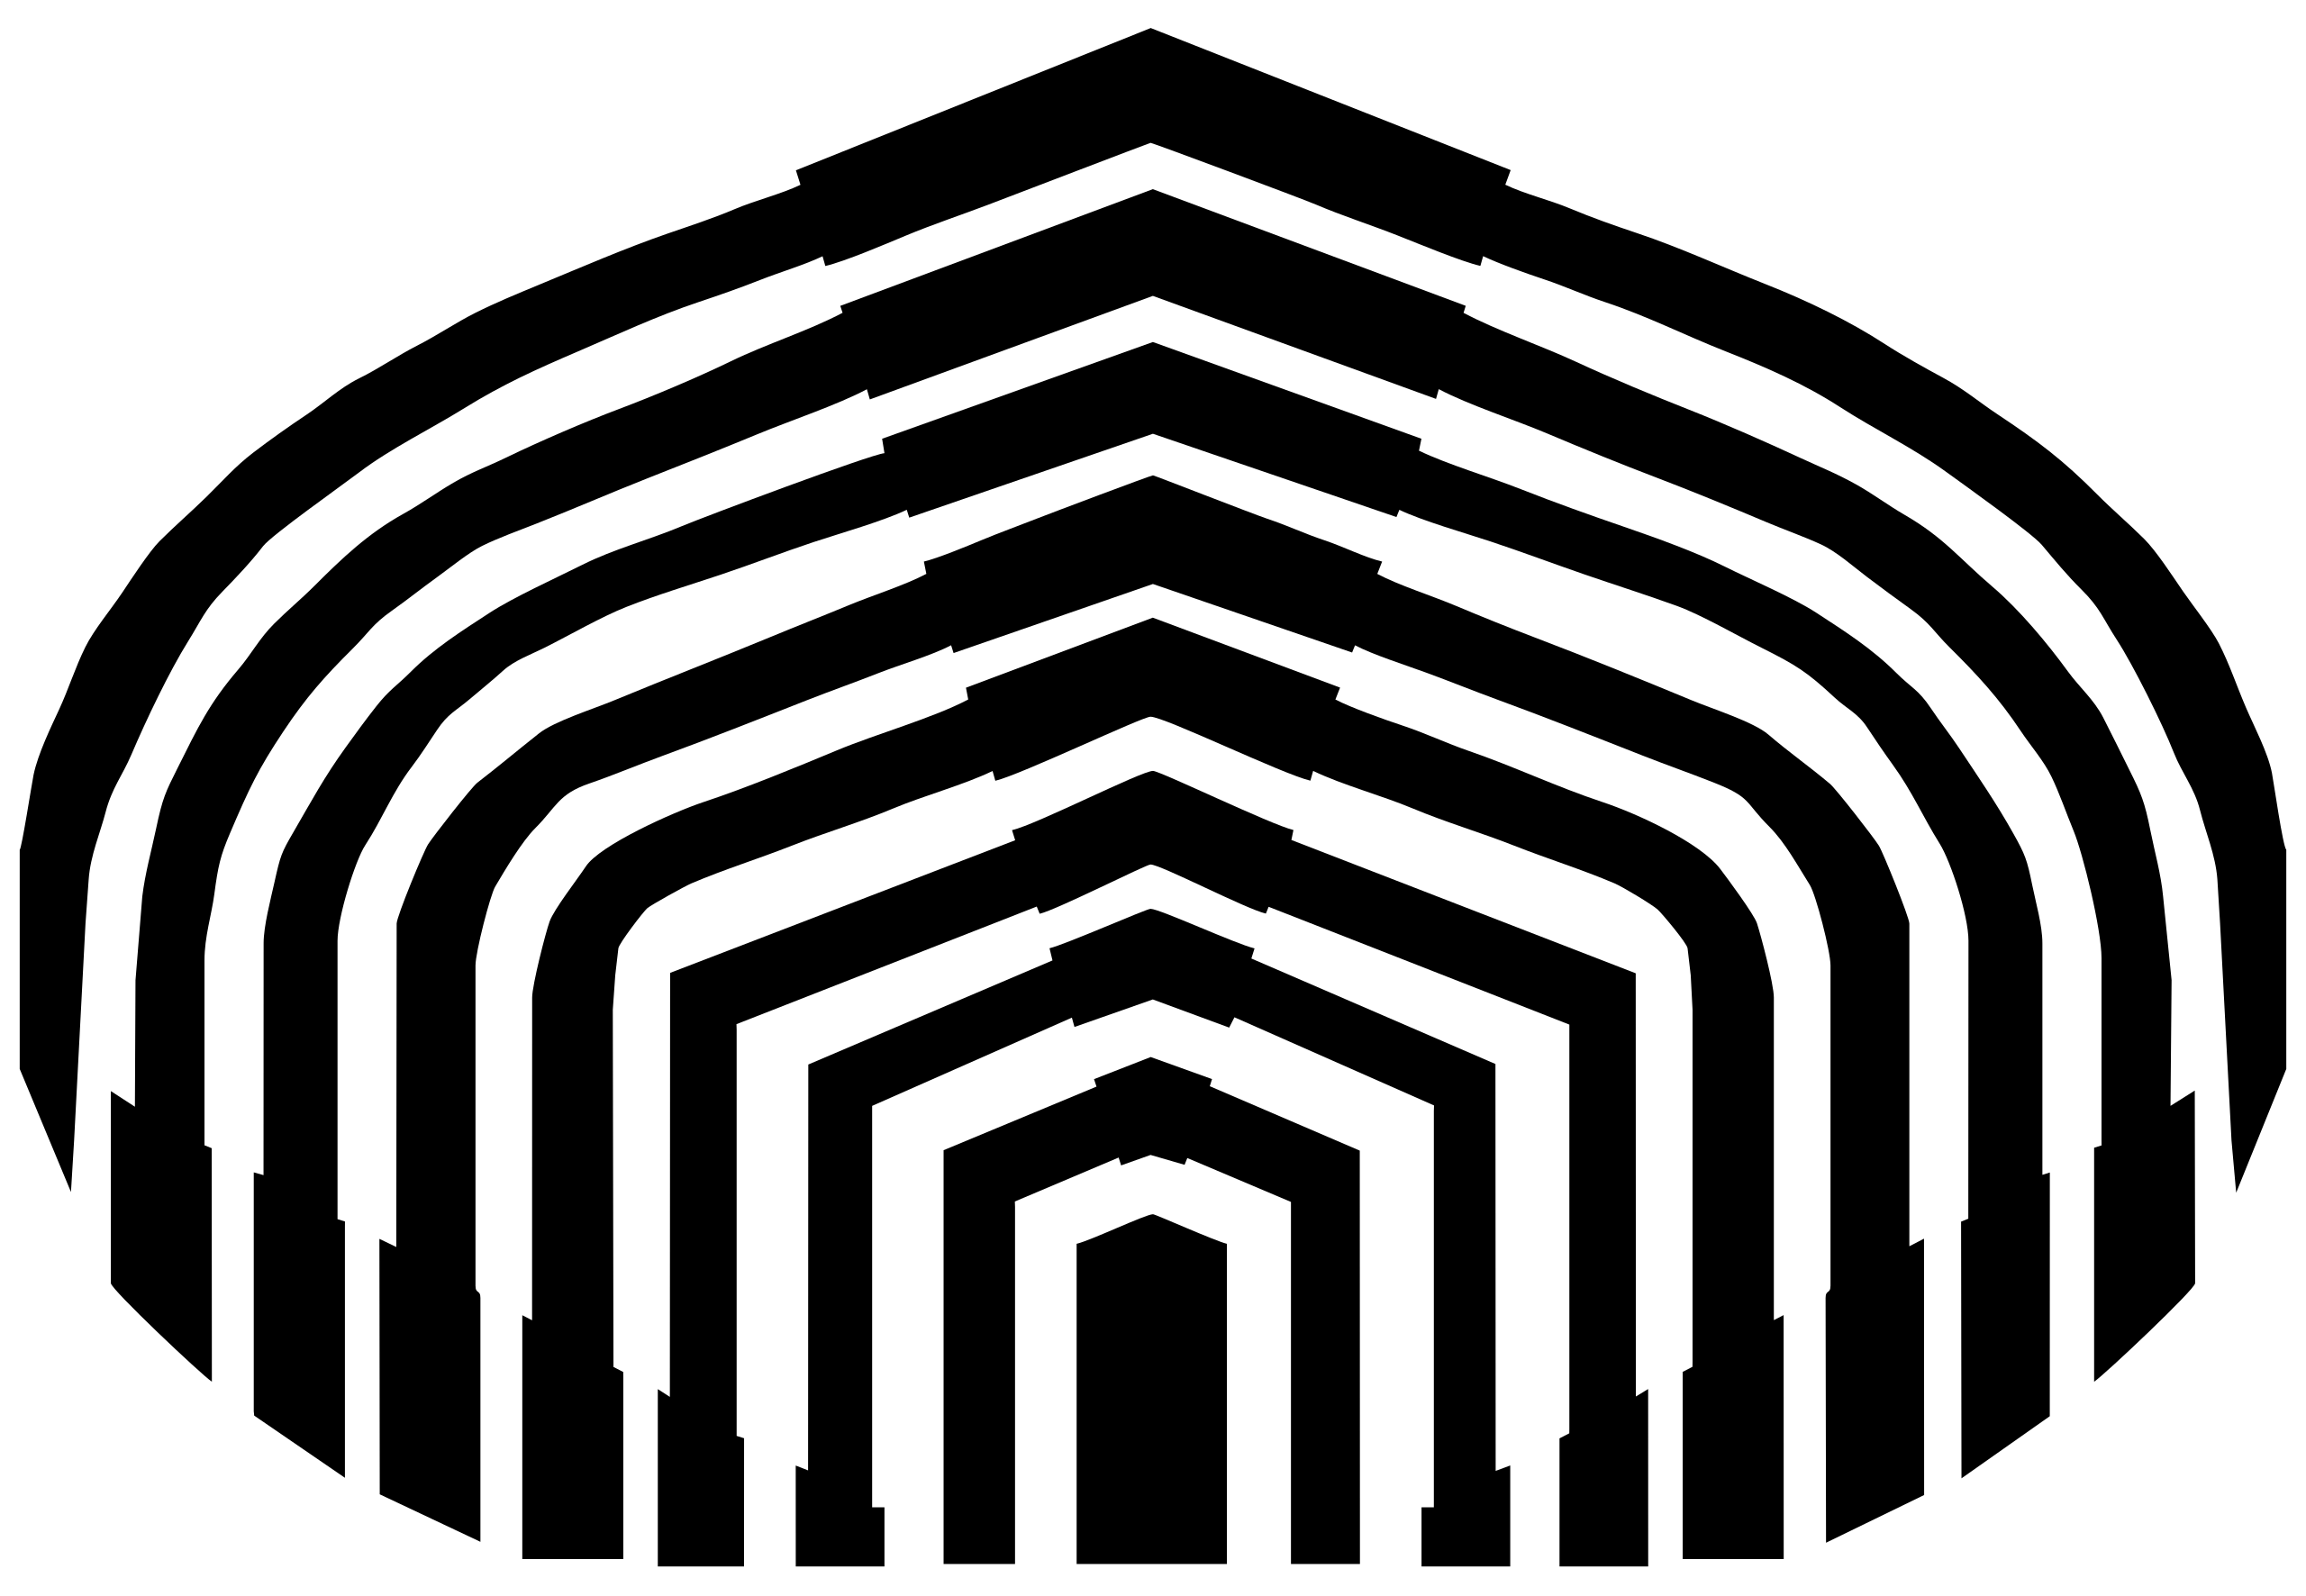
\includegraphics[width=3.1cm,height=2cm]{logo}\\
		UNIVERSIDAD SIMÓN BOLÍVAR\\
		DEPARTAMENTO DE ELECTRÓNICA Y CIRCUITOS\\
		EC1281 - LABORATORIO DE MEDICIONES ELÉCTRICAS\\
		SECCIÓN 1 - GRUPO 1\\
		
		\vspace{7cm}
		\textbf{\Large INFORME - PRÁCTICA \#3}\\
		PRINCIPIOS FUNDAMENTALES DE MEDICIONES ELÉCTRICAS INSTRUMENTOS DE MEDICIÓN PARA CORRIENTE DIRECTA (DC)\\
	\end{center}
	
	\begin{flushleft}
		\vspace{8cm}
		\hfill Integrantes:\\
		\hfill {\large Luis Becerra - 1910557}\\
		\hfill {\large Lorena Rojas - 1910469}\\
	\end{flushleft}
	
	\newpage
	
	\pagenumbering{roman}
	
	\begin{center}
		\textbf{\large RESUMEN}\\
	\end{center}
	
	En este laboratorio de mediciones eléctricas, el objetivo fue aplicar los conceptos fundamentales de medición y familiarizarnos con los instrumentos disponibles. Utilizamos un multímetro digital y analógico, voltímetro y amperímetro analógico. Realizamos mediciones de resistencia interna del amperímetro para cada una de las escalas, determinamos la linealidad en dos escalas y exploramos las características del voltímetro. Además, aprendimos sobre el puente de Wheatstone y realizamos mediciones de resistencias, comparando los resultados obtenidos con el multímetro digital y analógico. Observamos diferencias en las mediciones indirectas y se nos enfatizó estar atentos a estas discrepancias. En conclusión, esta práctica nos permitió adquirir experiencia en la utilización de los instrumentos de medición y comprender la importancia de la precisión y la calibración de los mismos.\\
		
	\newpage
	
	\begin{center}
		\textbf{\large ÍNDICE}\\
	\end{center}
	
	\noindent \textbf{RESUMEN} \hfill \textbf{I}\\
	\noindent \textbf{ÍNDICE} \hfill \textbf{II}\\
	\noindent \textbf{MARCO TEÓRICO} \hfill \textbf{1}\\
	\noindent \textbf{METEDOLOGÍA} \hfill \textbf{4}\\
	\noindent \textbf{RESULTADOS} \hfill \textbf{5}\\
	\noindent \textbf{ANÁLISIS DE RESULTADOS} \hfill \textbf{13}\\
	\noindent \textbf{CONCLUSIONES} \hfill \textbf{14}\\
	\noindent \textbf{BIBLIOGRAFÍA} \hfill \textbf{15}\\
	\noindent \textbf{ANEXOS} \hfill \textbf{16}\\
	
	\newpage
	
	\pagenumbering{arabic}
	
	\begin{center}
		\textbf{\large MARCO TEÓRICO}\\
	\end{center}
	
	\textbf{1. Conceptos fundamentales de medición y tipos de errores}\\
	
	En el campo de las mediciones eléctricas, es esencial comprender los conceptos básicos relacionados con los tipos y métodos de medición, así como los posibles errores que pueden surgir durante el proceso.\\
	
	La medición es el proceso de determinar el valor de una magnitud física utilizando instrumentos y técnicas específicas. Existen dos tipos principales de mediciones: directa e indirecta. La medición directa implica la lectura directa de un instrumento para obtener el valor de la magnitud, como medir la corriente con un amperímetro. Por otro lado, la medición indirecta implica el cálculo o la combinación de varias mediciones para obtener el valor deseado, como determinar la resistencia utilizando el método del puente de Wheatstone.\\
	
	Durante el proceso de medición, es importante tener en cuenta los posibles errores que pueden afectar la precisión y exactitud de los resultados. Los errores pueden clasificarse en varias categorías:\\
	
	\begin{itemize}
		\item Los \textbf{errores grandes} son aquellos que resultan en mediciones significativamente diferentes al valor verdadero, generalmente causados por fallos en el equipo o en el procedimiento experimental. Estos errores pueden evitarse siguiendo cuidadosamente las instrucciones y verificando el buen estado de los instrumentos antes de su uso.\\
	
		\item Los \textbf{errores sistemáticos} son aquellos que ocurren de manera consistente y predecible, como los errores del instrumento, del método utilizado, por condiciones ambientales o de observación. Por ejemplo, un instrumento de medición puede tener una desviación sistemática que afecta todas las mediciones realizadas con él. Para evitar o corregir estos errores, es necesario calibrar y verificar periódicamente los instrumentos, utilizar métodos adecuados y considerar las condiciones ambientales durante las mediciones.\\
	
		\item Y por ultimo los \textbf{errores aleatorios} son impredecibles y pueden deberse a fluctuaciones en las mediciones o a la variabilidad inherente del sistema. Estos errores pueden minimizarse mediante el uso de técnicas de promediado y tomando múltiples mediciones. Además, es importante tener en cuenta la incertidumbre asociada a cada medición y expresar los resultados de manera adecuada, utilizando cifras significativas y notación científica cuando sea necesario.\\
	
	\end{itemize}
	
	En resumen, el proceso de medición implica la selección adecuada de los métodos y instrumentos de medición, así como la consideración de los posibles errores que pueden surgir. La comprensión de los tipos de errores y los procedimientos para evitarlos o corregirlos es fundamental para obtener resultados confiables y precisos en las mediciones eléctricas.
	
	\textbf{2. Galvanómetro de D'Arsonval}\\
	
	El Galvanómetro de D'Arsonval es un instrumento electromecánico utilizado como base para la construcción de amperímetros y voltímetros analógicos. Fue inventado por el físico francés Jacques-Arsène d'Arsonval en el siglo XIX.\\
	
	El principio de operación del Galvanómetro de D'Arsonval se basa en la interacción entre un campo magnético y una corriente eléctrica. Consiste en una bobina móvil suspendida entre los polos de un imán permanente. Cuando circula una corriente eléctrica a través de la bobina, se genera un campo magnético que interactúa con el campo magnético del imán, lo que produce una fuerza proporcional a la corriente. Esta fuerza hace que la bobina se desplace y se deflexione en proporción a la corriente medida.\\
	
	Los amperímetros y voltímetros analógicos se construyen utilizando el Galvanómetro de D'Arsonval como base. En el caso de los amperímetros, se conecta una resistencia en paralelo a la bobina móvil para limitar la corriente máxima que puede circular por el instrumento. Esto permite medir la corriente que circula por un circuito sin interrumpirlo significativamente. Para los voltímetros, se coloca una resistencia en serie con la bobina para crear una caída de voltaje proporcional a la corriente. De esta manera, se puede medir el voltaje en un circuito sin alterar significativamente la corriente.\\
	
	Estos instrumentos analógicos se caracterizan por tener una escala graduada que permite leer directamente el valor de la magnitud medida. La precisión y resolución de estos instrumentos dependen de la sensibilidad, la gama y la linealidad del sistema. La sensibilidad se refiere a la cantidad mínima de corriente o voltaje que puede ser detectada por el instrumento. La gama es el rango de valores que el instrumento puede medir. La linealidad se refiere a la relación lineal entre la deflexión del galvanómetro y la magnitud medida.\\
	
	En conclusión, el Galvanómetro de D'Arsonval es la base para la construcción de amperímetros y voltímetros analógicos. Estos instrumentos aprovechan el principio de interacción entre un campo magnético y una corriente eléctrica para realizar mediciones eléctricas. Comprender el principio de construcción de estos instrumentos es fundamental para su correcta utilización en las mediciones eléctricas.\\
	
	\newpage
	
	\begin{center}
		\textbf{\large METODOLOGÍA}\\
	\end{center}

	En la metodología del laboratorio de mediciones eléctricas, se utilizaron diversos circuitos y procedimientos de medición para obtener información relevante. A continuación, se describen brevemente los circuitos y procedimientos utilizados para cada objetivo:\\
	
	\begin{enumerate}
		\item \textbf{Medición de la resistencia interna de las escalas del amperímetro:}
		
		\begin{itemize}
			\item Se conectó el amperímetro en serie con el multimetro digital, una resistencia de protección para el multimetro y una fuente de corriente constante.
			\item Se seleccionó una escala específica del amperímetro y establecio un voltaje especifico que mostrara una lectura tanto en el multimetro digital como el amperímetro.
			\item Con dicho valor de la fuente, se sustituyó el amperímetro por una década de resistencia y se estableció un valor hasta obtener la misma lectura en el multimetro antes obtenida. 
			\item Se repitió el procedimiento para cada escala del amperímetro, registrando los valores de voltaje y resistencia obtenidos.
		\end{itemize}
		
		\item \textbf{Determinación de la resistencia interna de un voltímetro:}
		
		\begin{itemize}
			\item Se determina utilizando la característica $\Omega V$ proporcionada por el fabricante. Para nuestro voltímetro fue $10K\Omega V$
			\item Para cada escala, se multiplicó el máximo de la
			escala por la característica $\Omega V$ para obtener la correspondiente resistencia interna mediante la siguiente fórmula: $R_{volt1} = R_{i} + R_{1} = Y(\Omega V) * E_{max}$ 
		\end{itemize}
		
		\item \textbf{Medición del valor real de las resistencias bajo prueba:}
		
		\textbf{3.1. Método del puente de Wheatstone:}
		
		\begin{itemize}
			\item Se armó un circuito de puente de Wheatstone con la resistencia bajo prueba, una resistencia conocida, y resistencias variables.
			\item Se ajustaron las resistencias variables hasta lograr un equilibrio en el puente, donde no circulaba corriente a través del galvanómetro.
			\item Se registraron los valores de las resistencias utilizadas para alcanzar el equilibrio.
			\item Utilizando la relación de equilibrio del puente de Wheatstone, se calculó el valor real de la resistencia bajo prueba.
		\end{itemize}
		
		\textbf{3.2. Mediciones indirectas:}
		
		\begin{itemize}
			\item Se construyó un circuito con el amperímetro y el voltímetro en serie con la resistencia bajo prueba.
			\item Se midieron los valores de corriente y voltaje en el circuito.
			\item Utilizando la ley de Ohm, se calculó el valor de la resistencia bajo prueba a partir de los valores medidos de corriente y voltaje.
		\end{itemize}
		
	\end{enumerate}
	
	Es importante destacar que se utilizaron componentes con valores nominales conocidos y se tomaron todas las precauciones necesarias para garantizar mediciones precisas y evitar daños en los instrumentos utilizados. Se realizaron múltiples mediciones y se promediaron los resultados para obtener valores más confiables.

	\newpage
	
	\begin{center}
		\textbf{\large RESULTADOS}\\
	\end{center}
	
	\noindent Durante las mediciones se obtuvieron los siguientes resultados:
	
	\begin{center}
		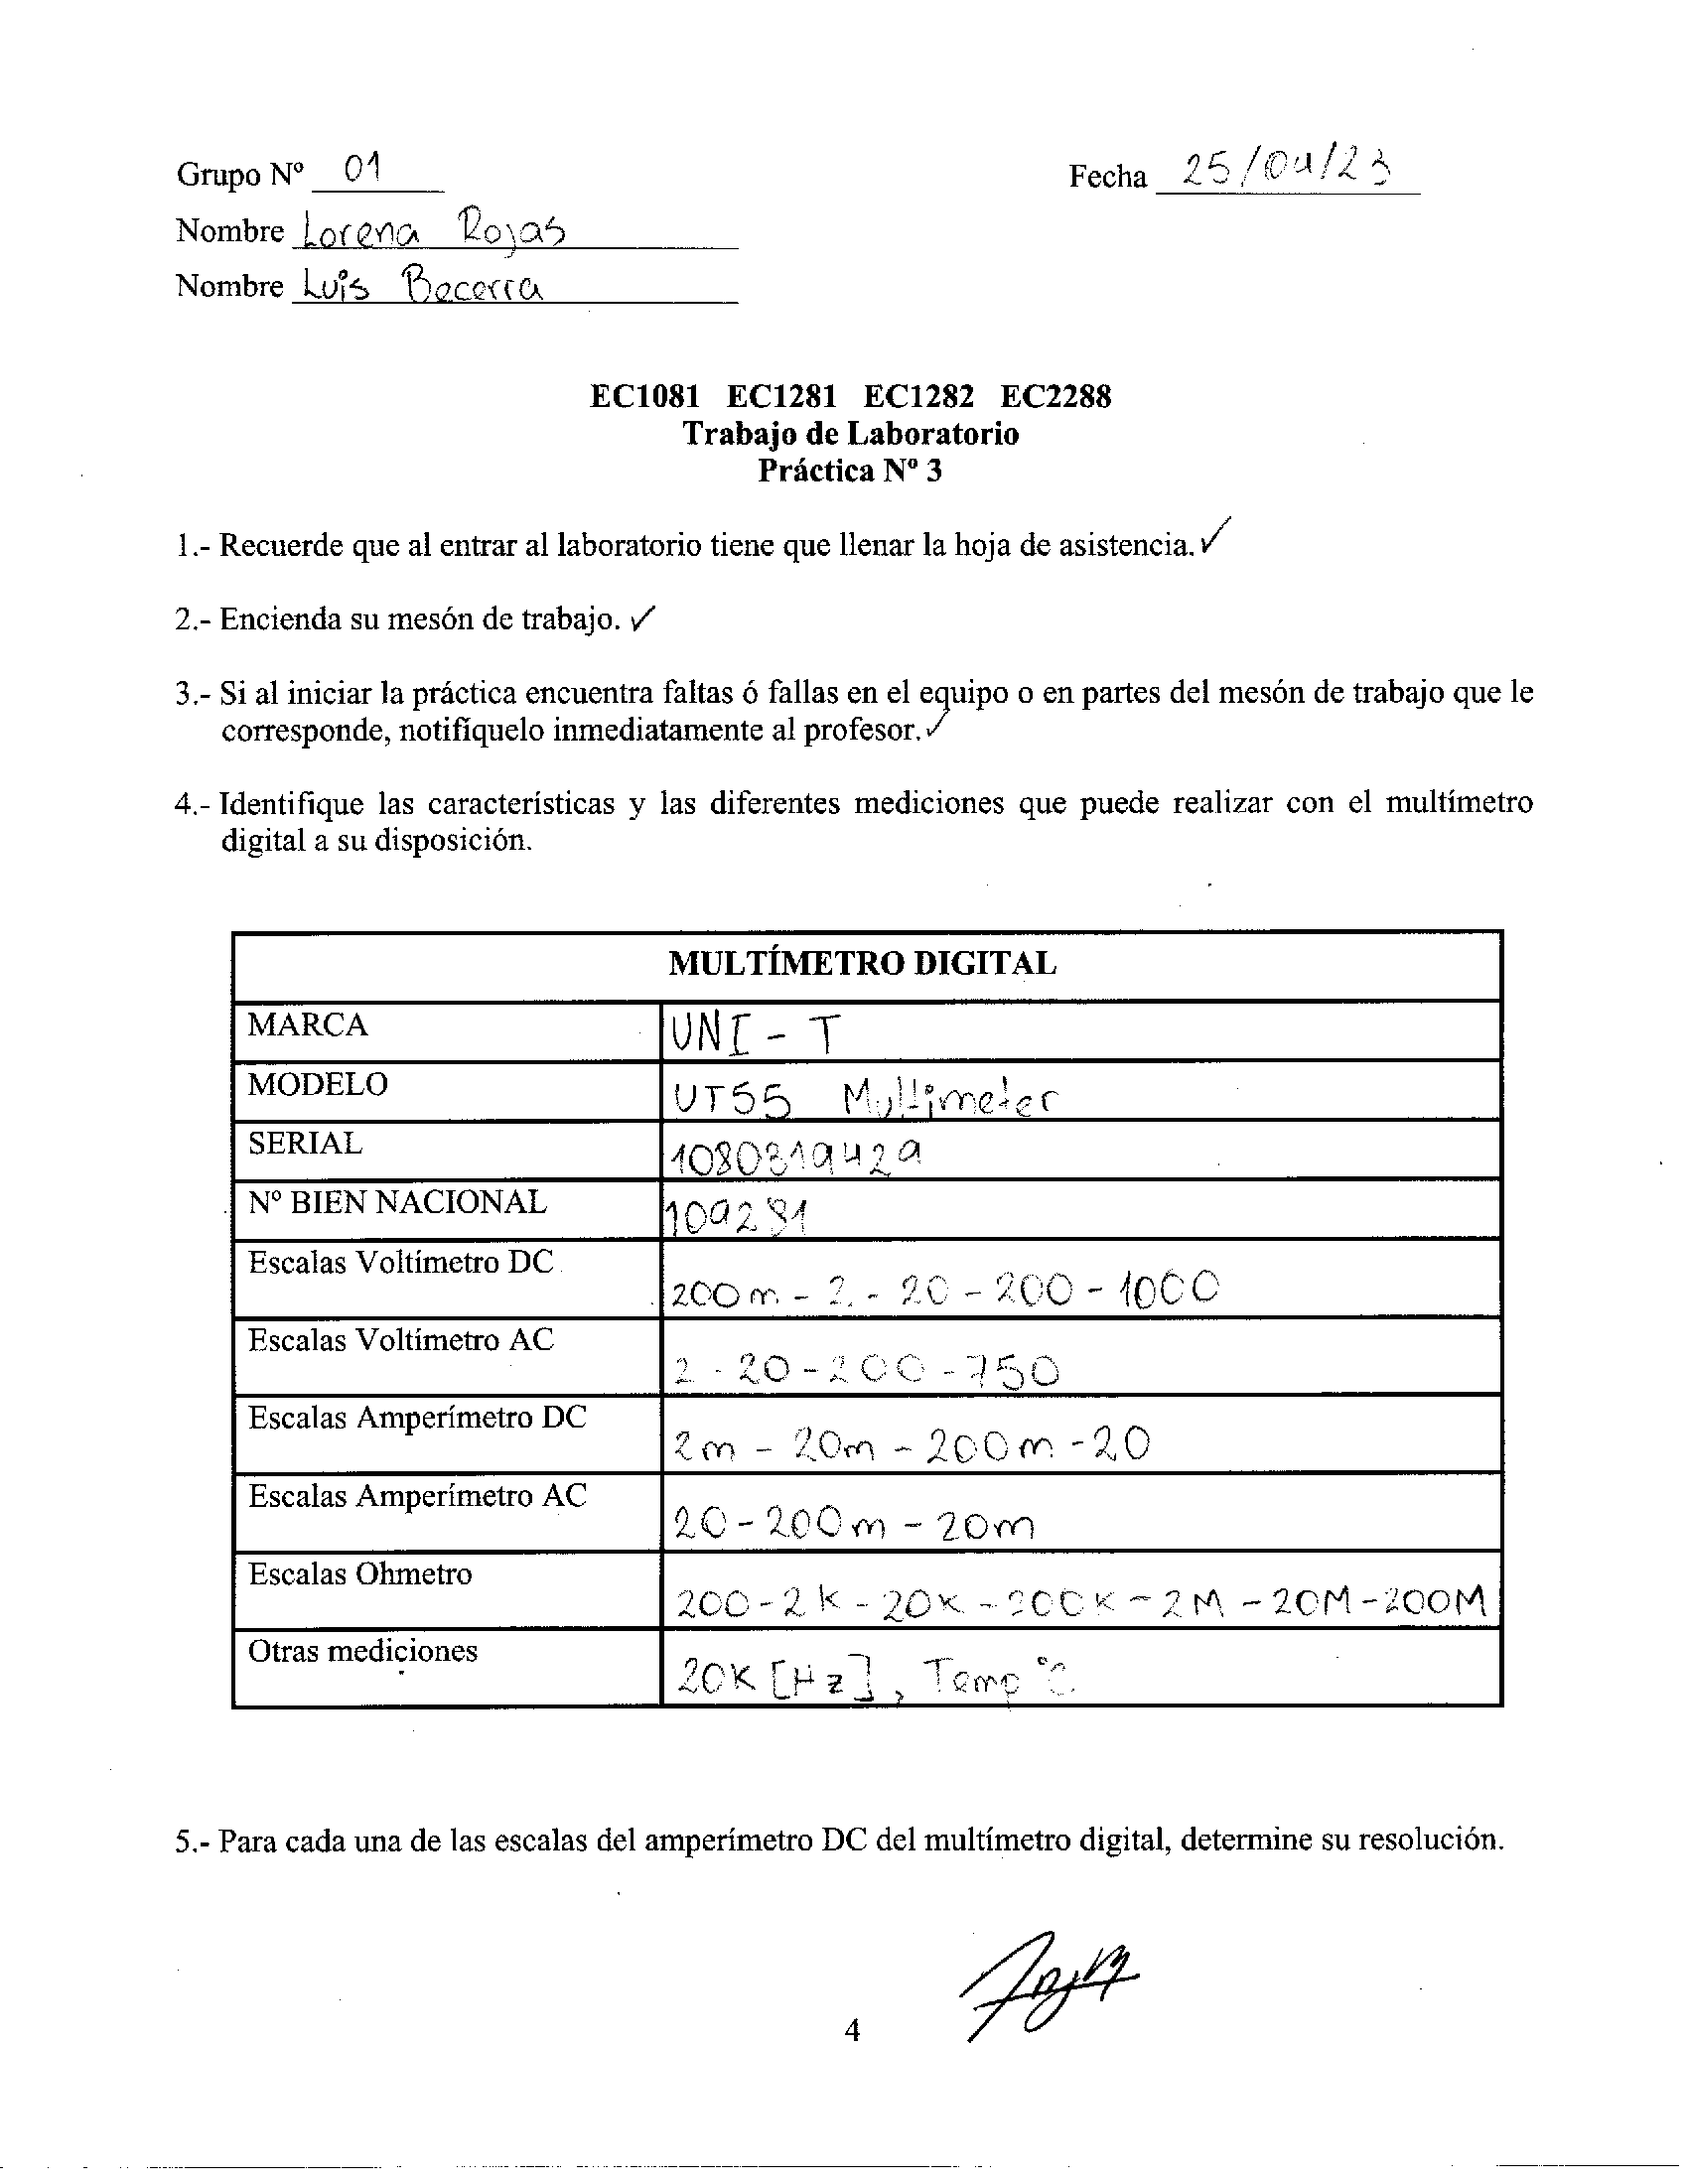
\includegraphics[width=16cm,height=20cm]{Img/datos_lab_0001}
	\end{center}

	\begin{center}
		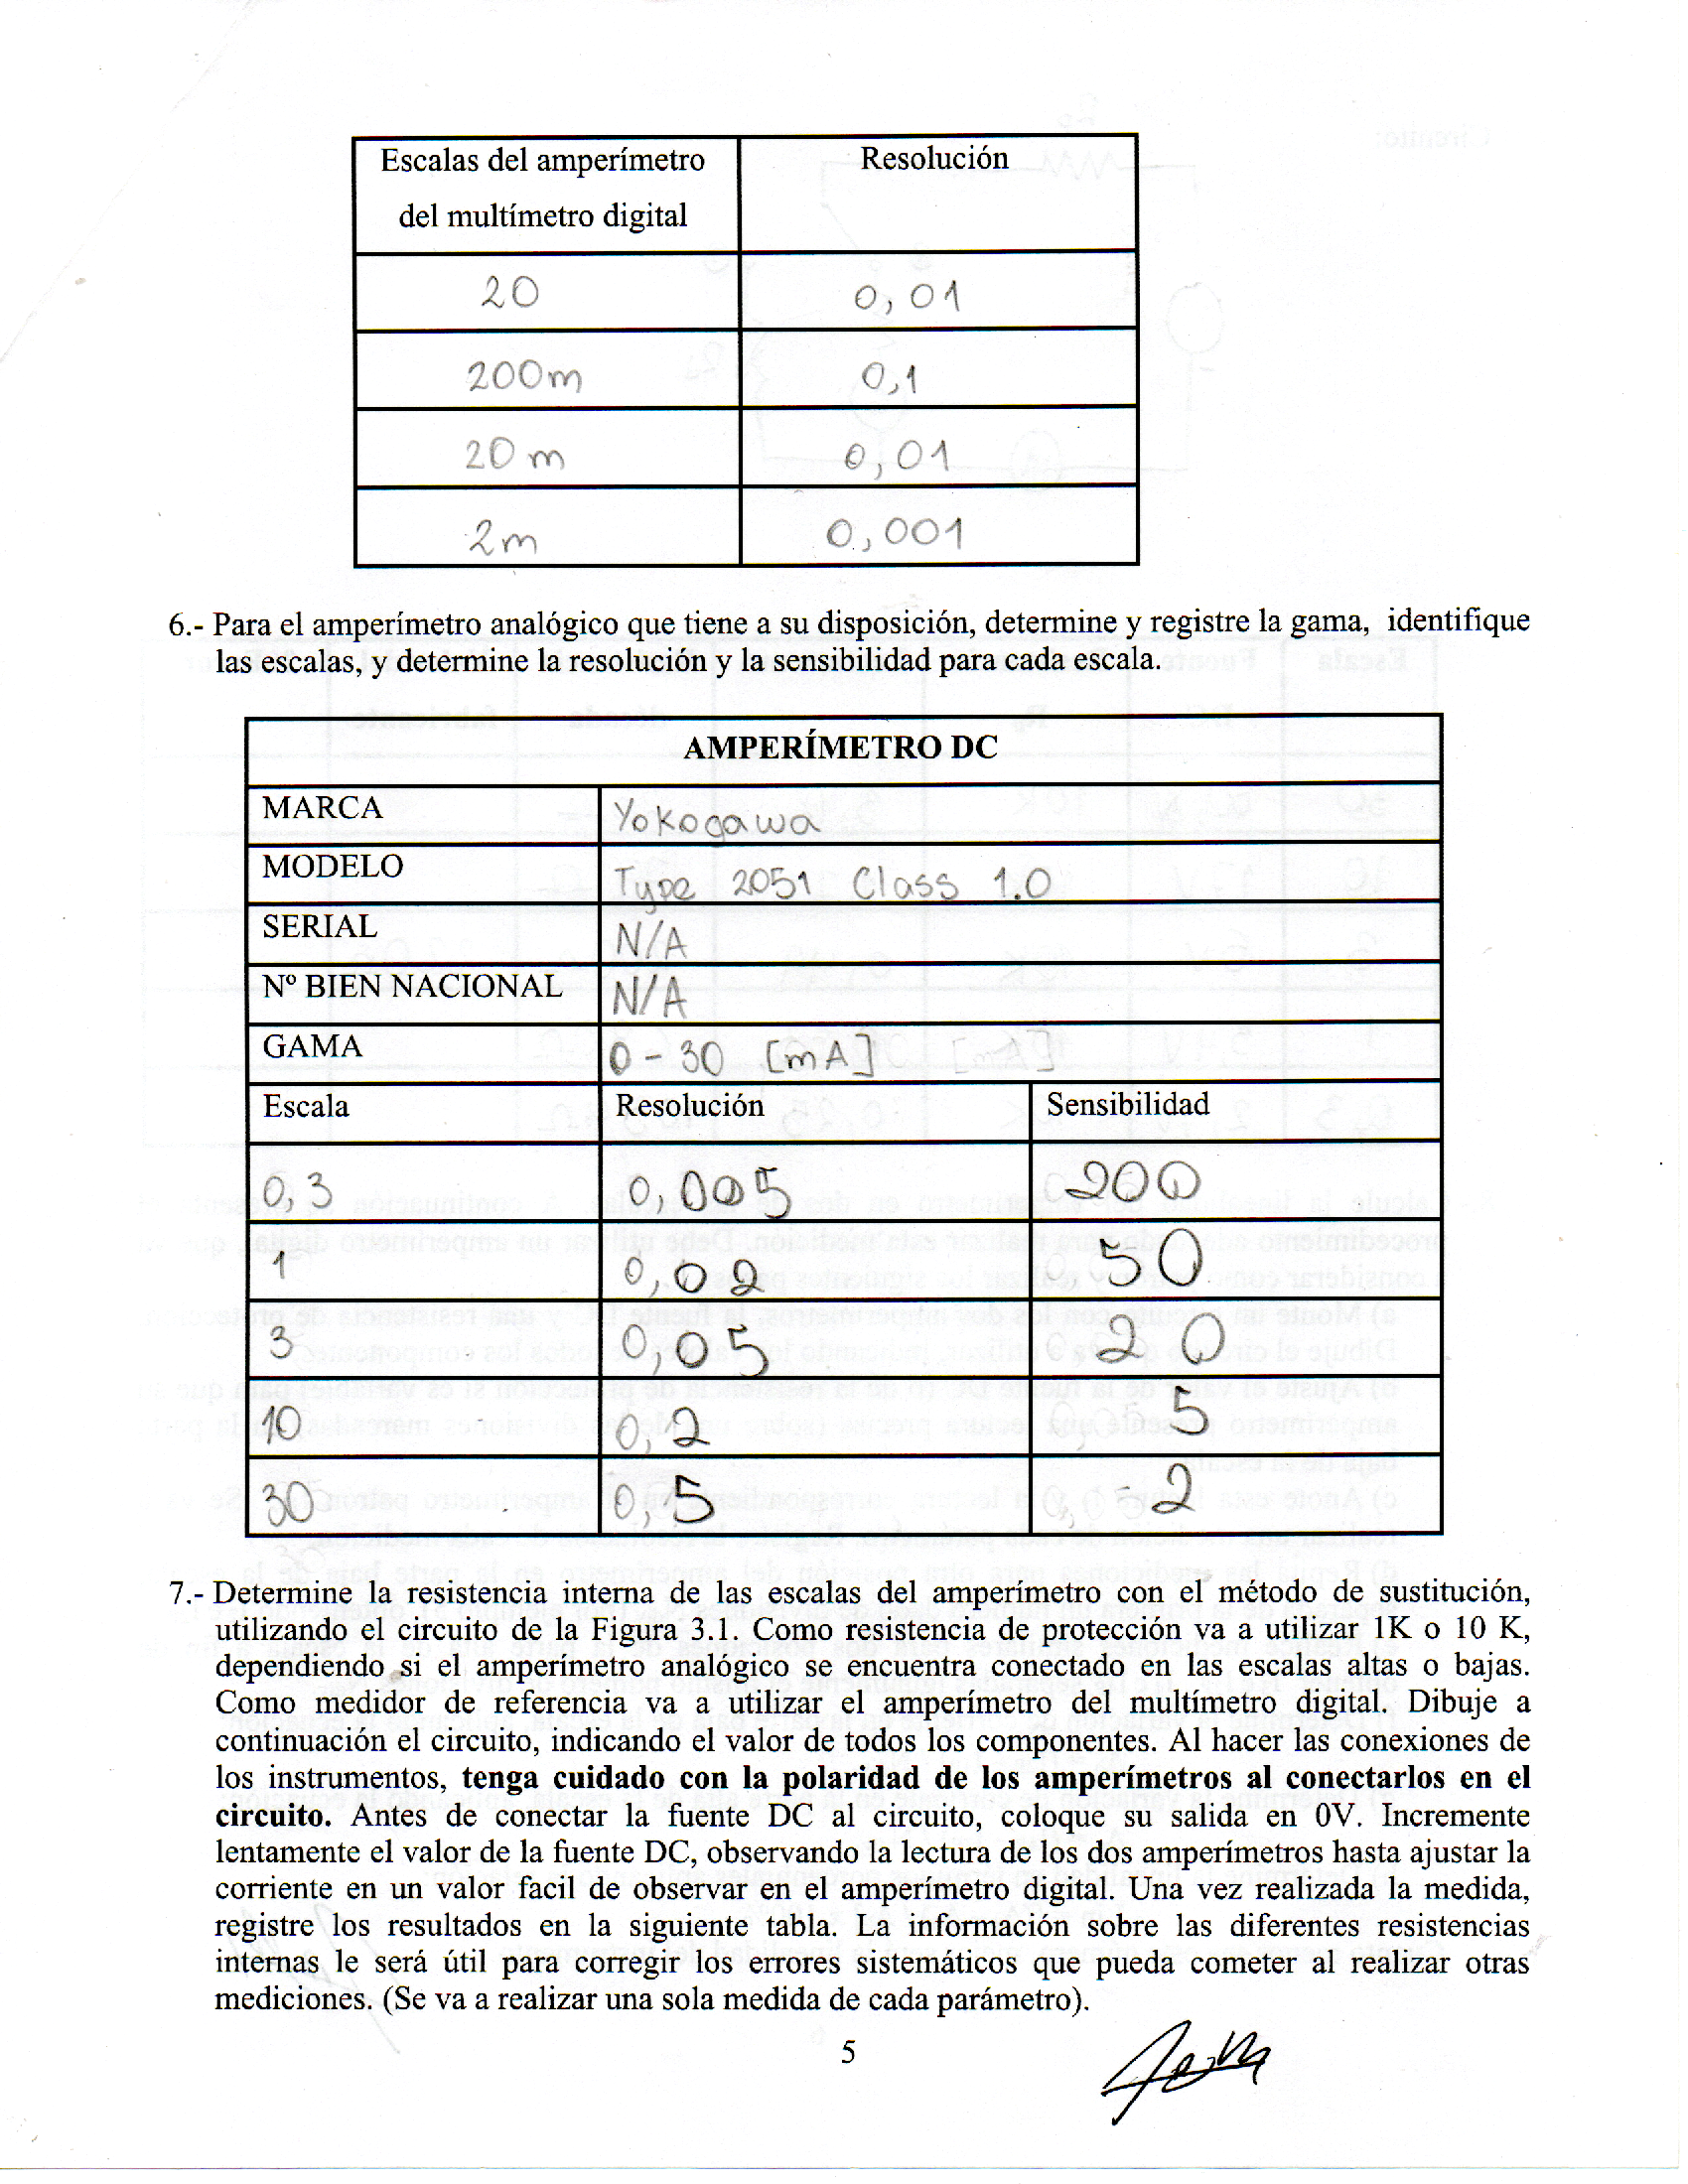
\includegraphics[width=16cm,height=20cm]{Img/datos_lab_0002}
	\end{center}
	
	\begin{center}
		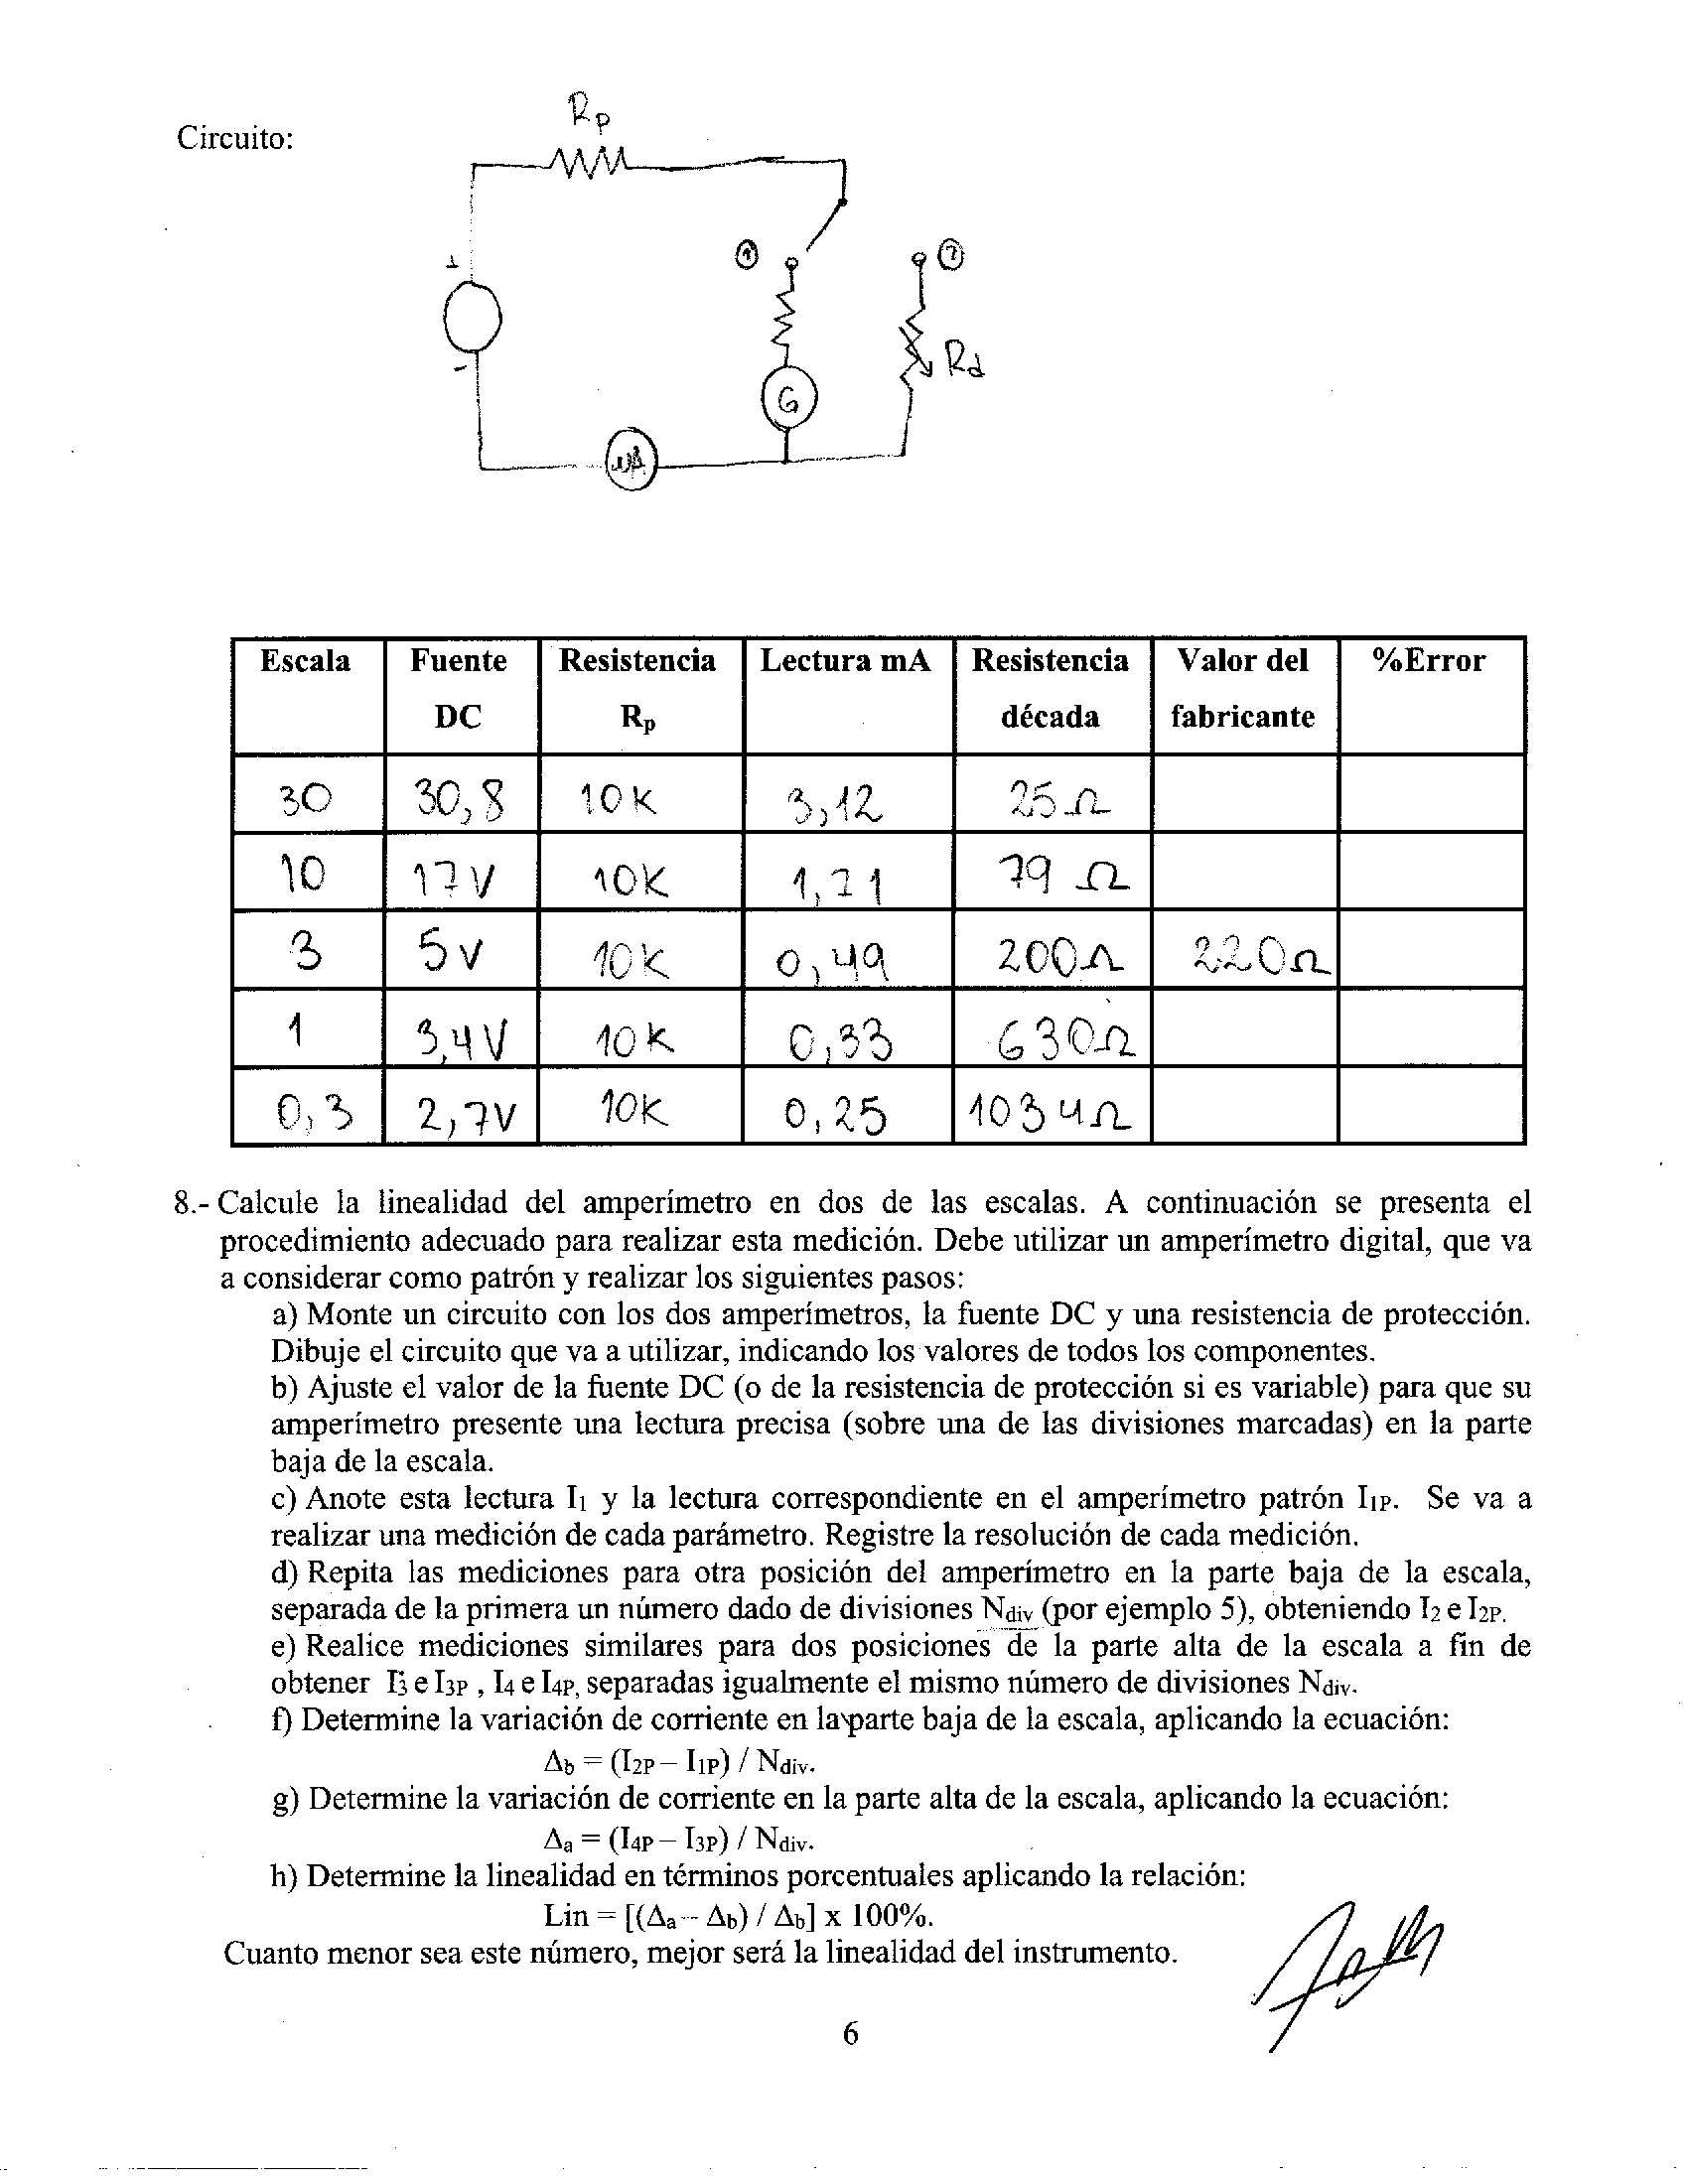
\includegraphics[width=16cm,height=20cm]{Img/datos_lab_0003}
	\end{center}

	\begin{center}
		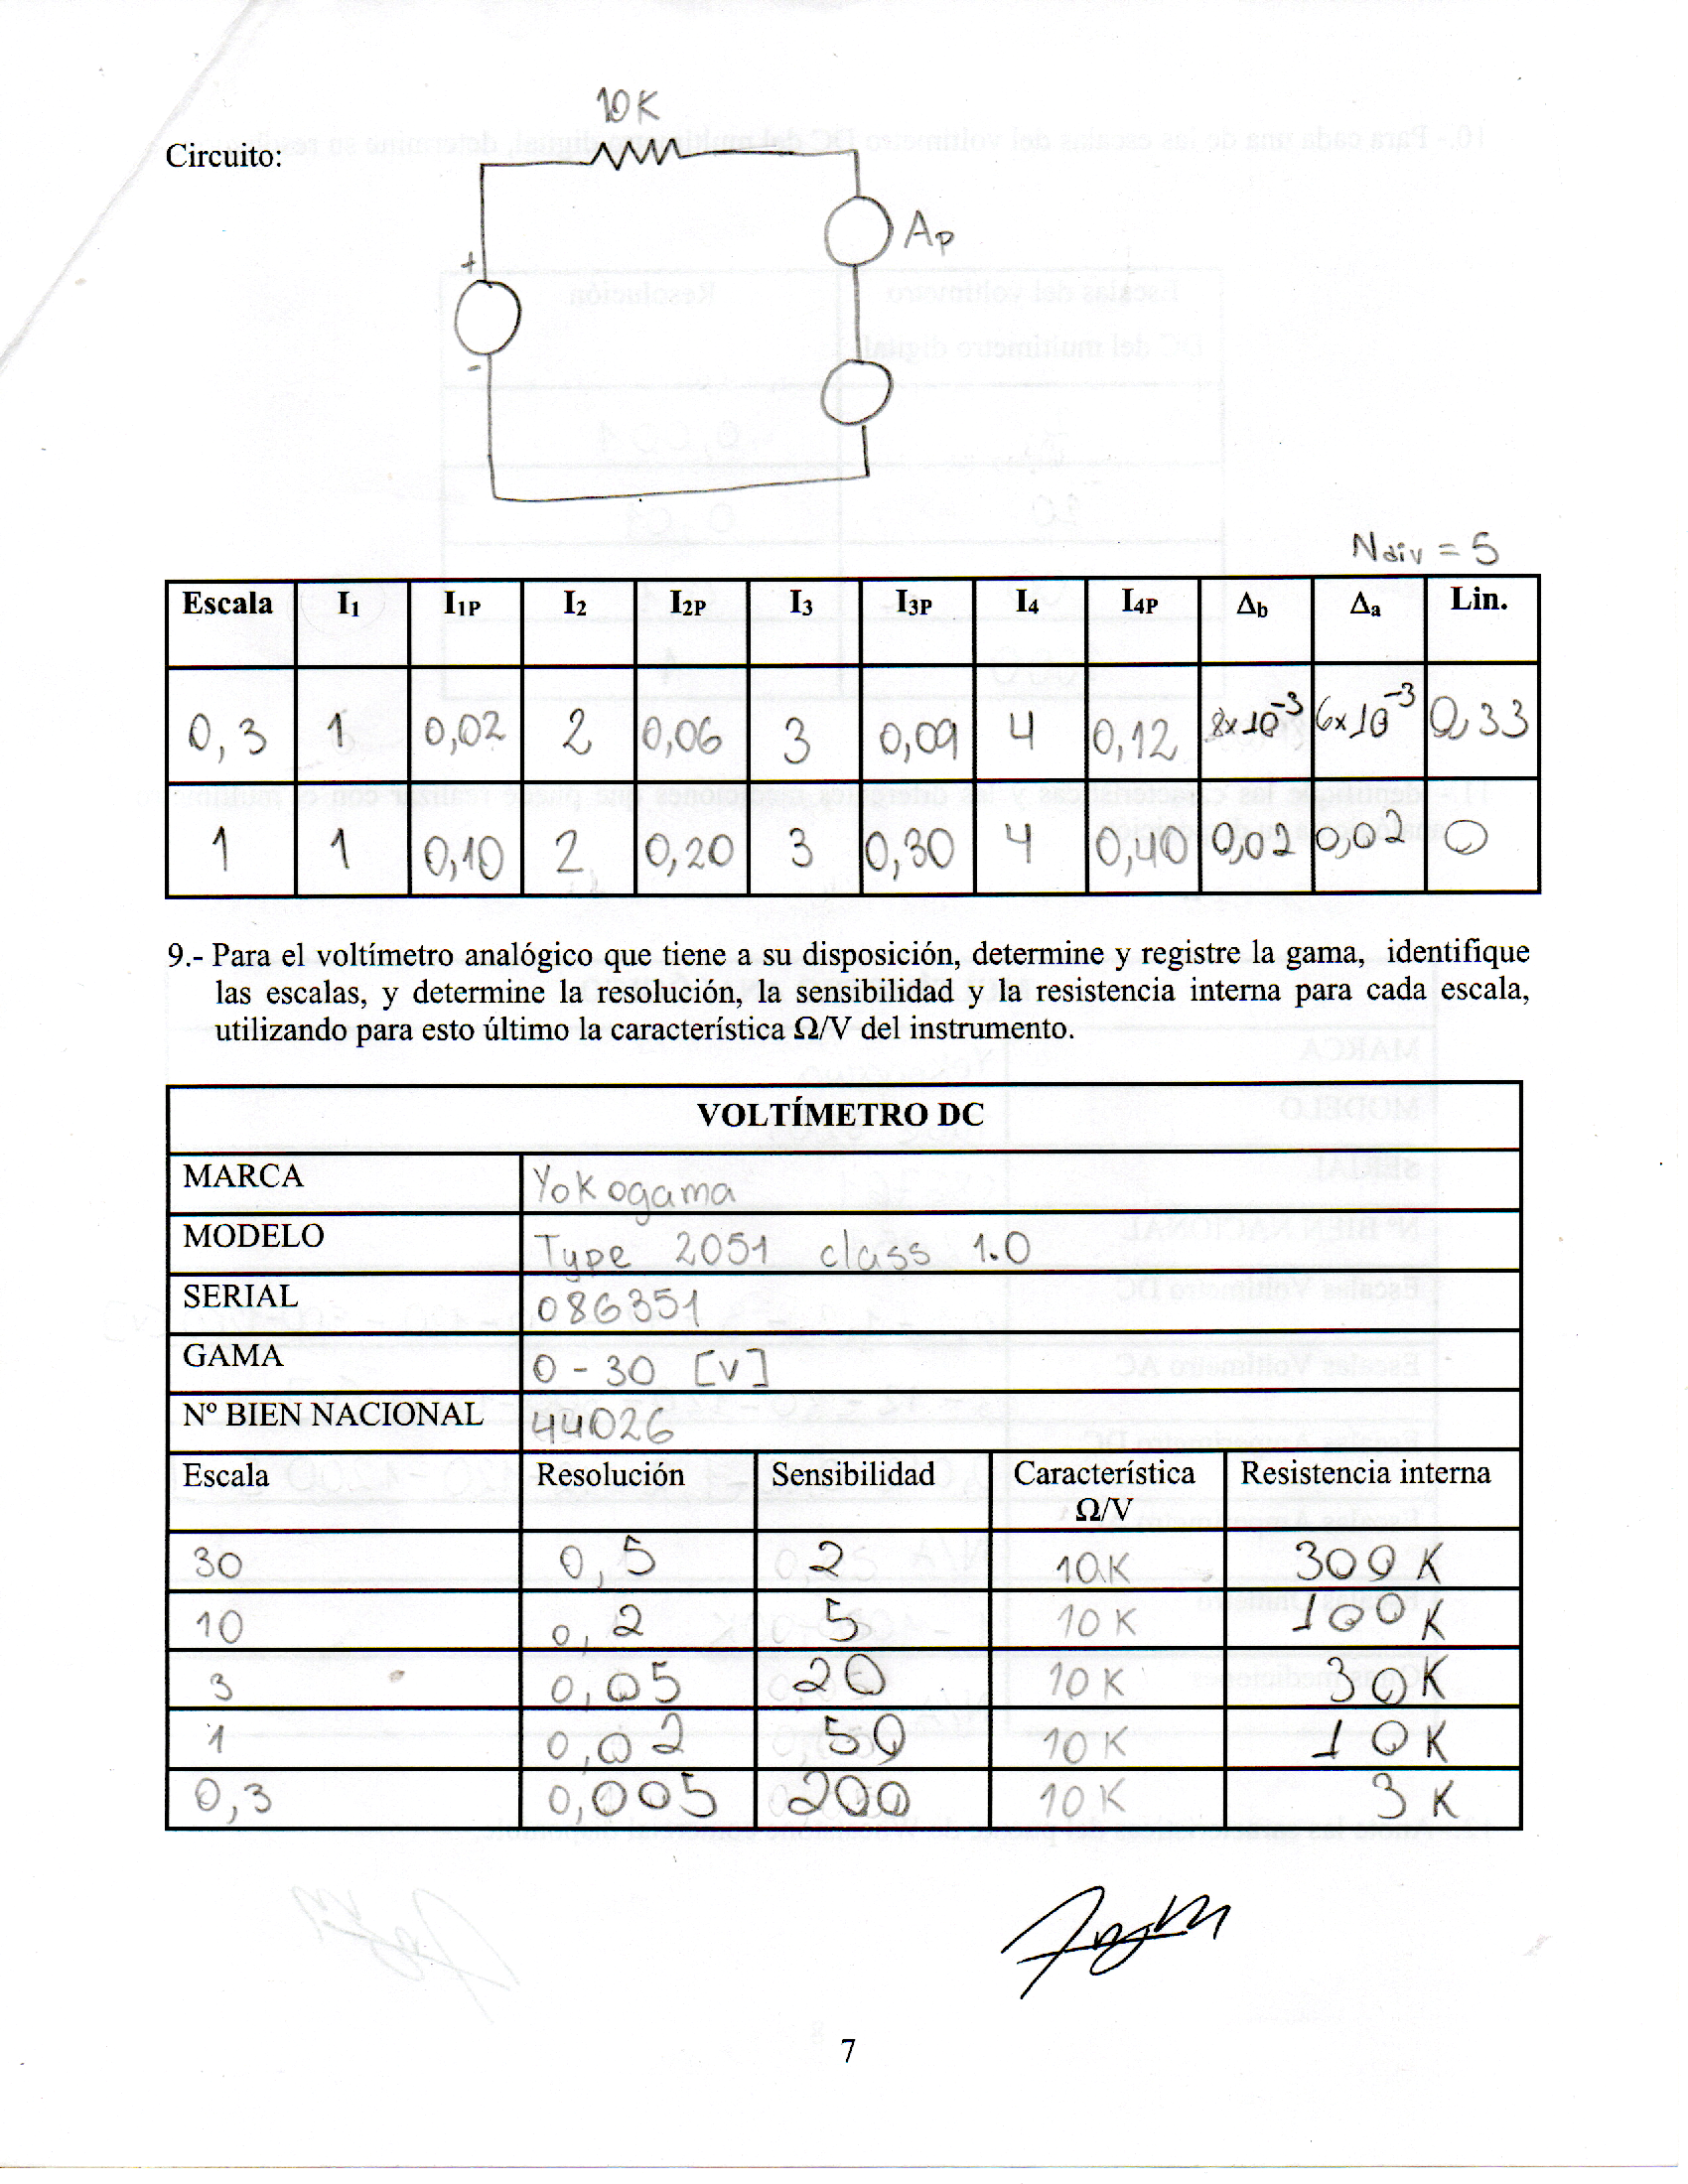
\includegraphics[width=16cm,height=20cm]{Img/datos_lab_0004}
	\end{center}

	\begin{center}
		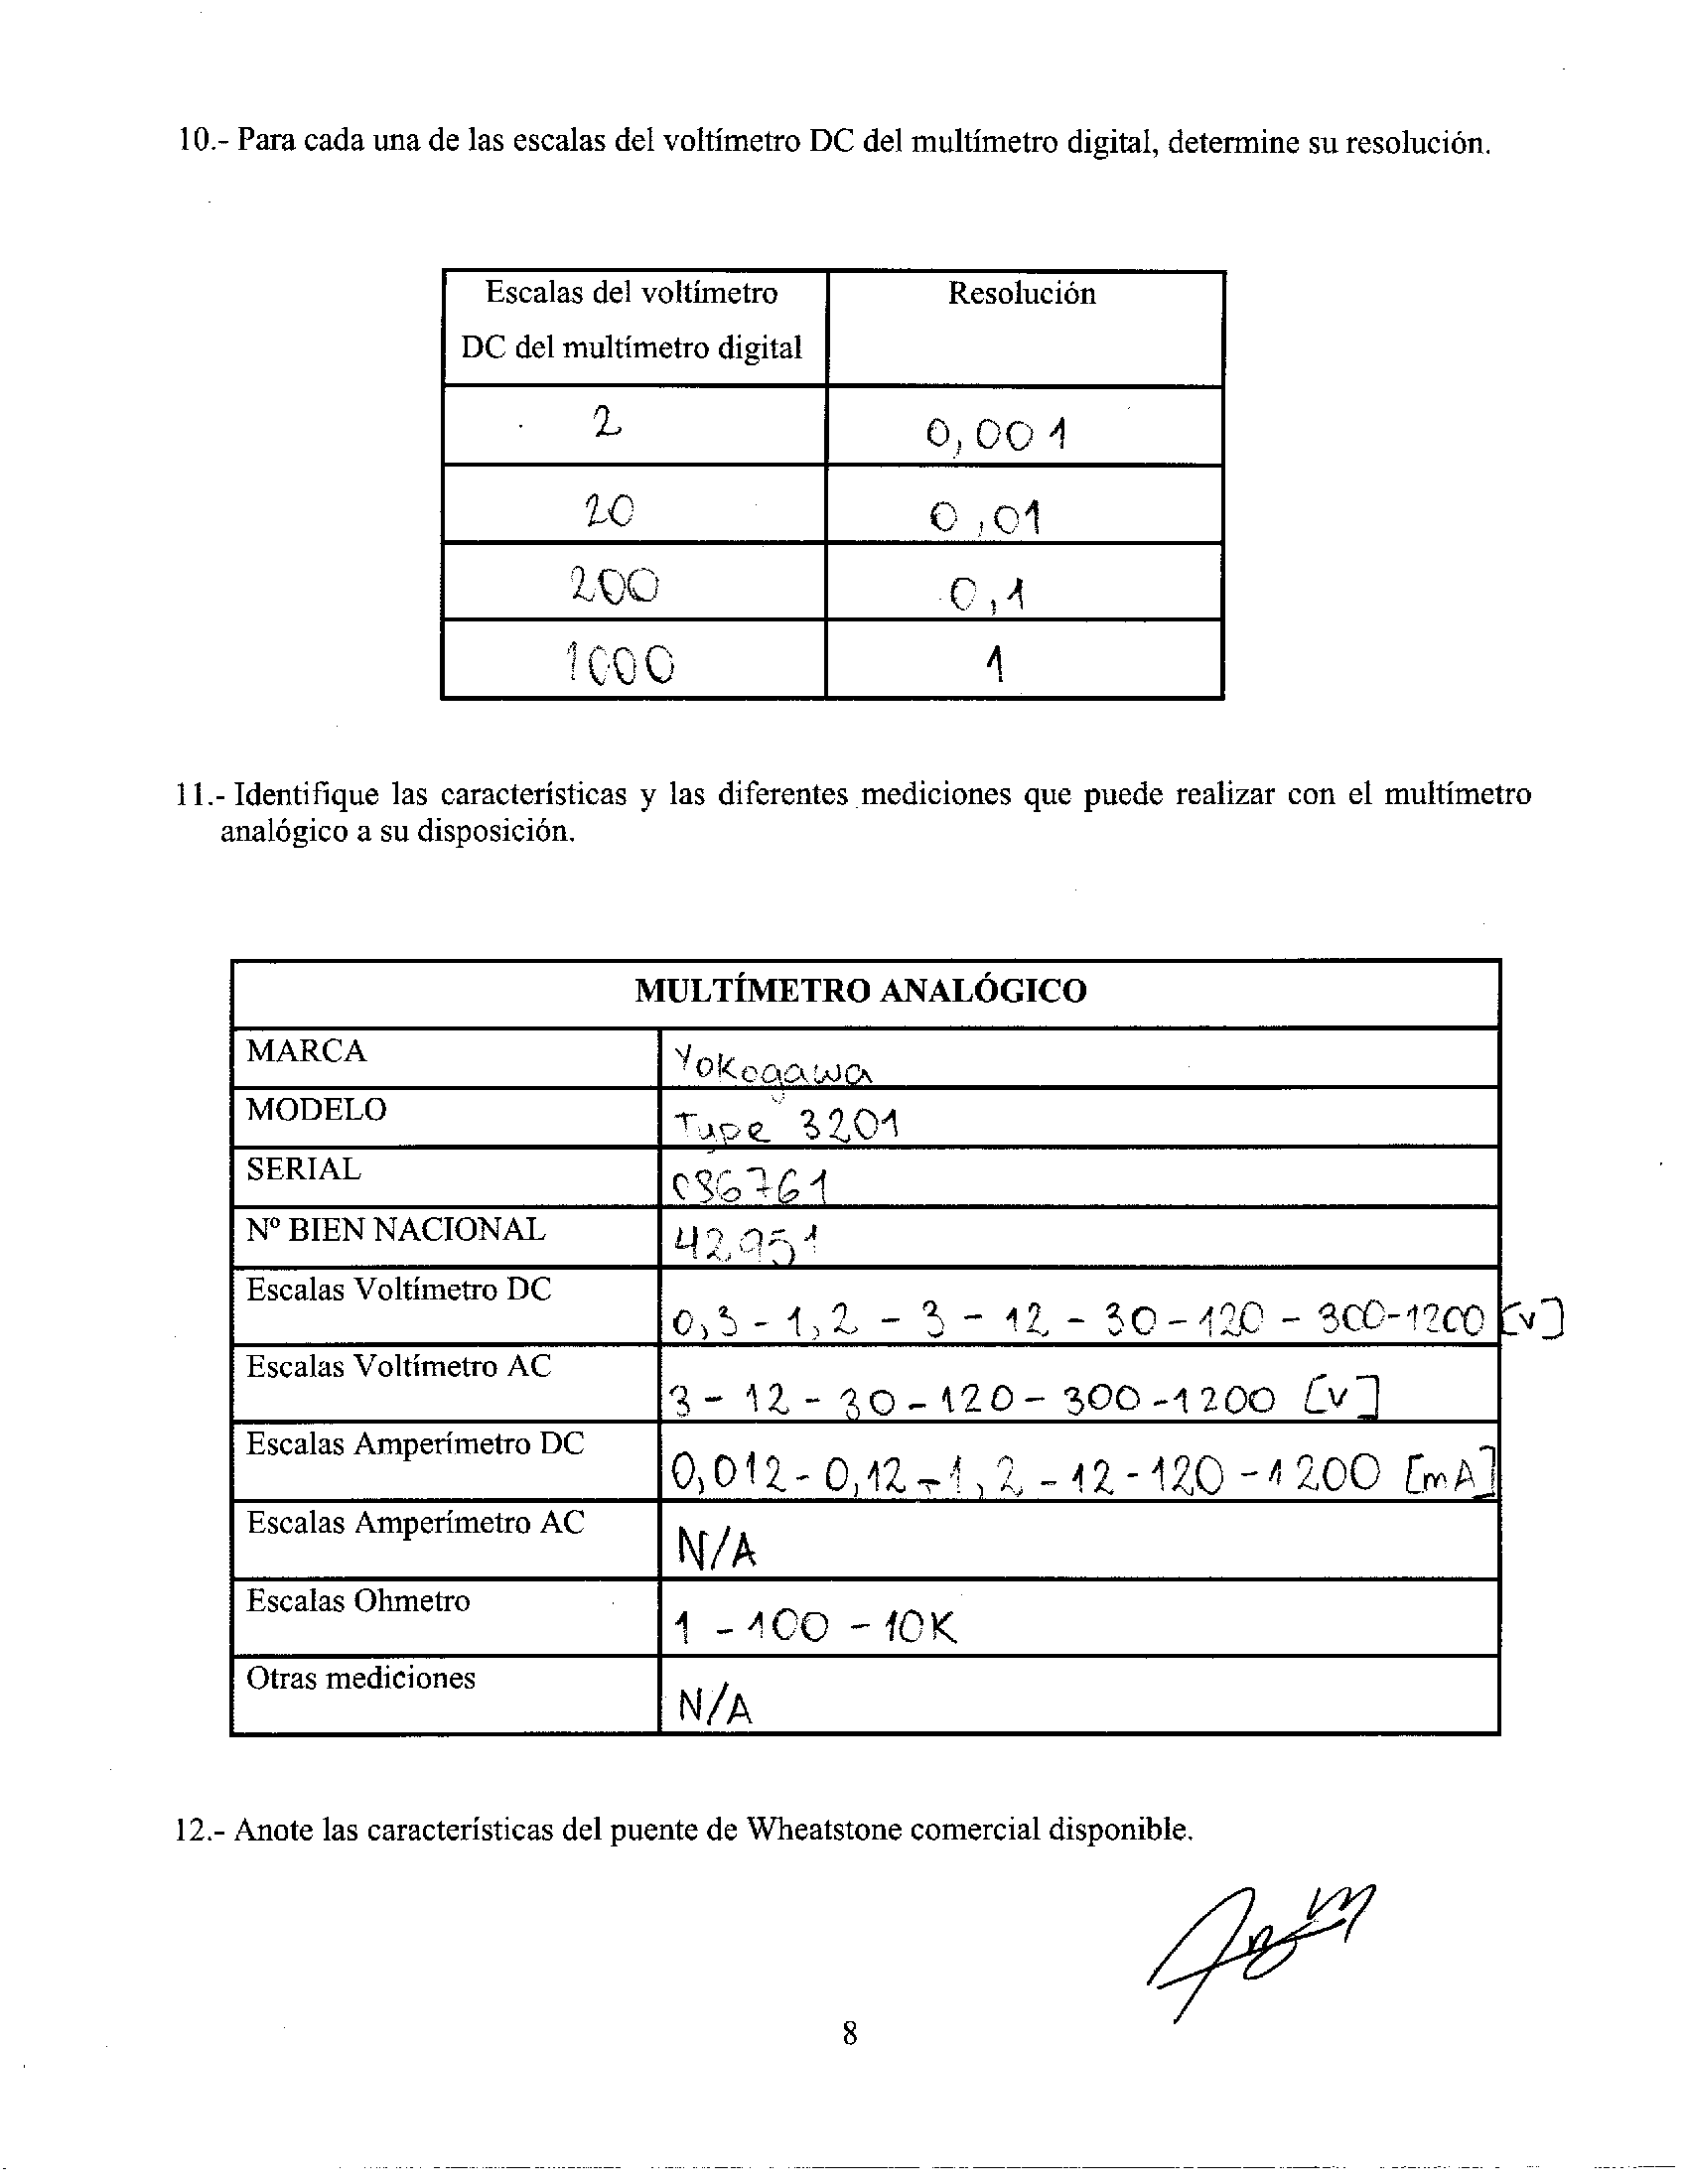
\includegraphics[width=16cm,height=20cm]{Img/datos_lab_0005}
	\end{center}

	\begin{center}
		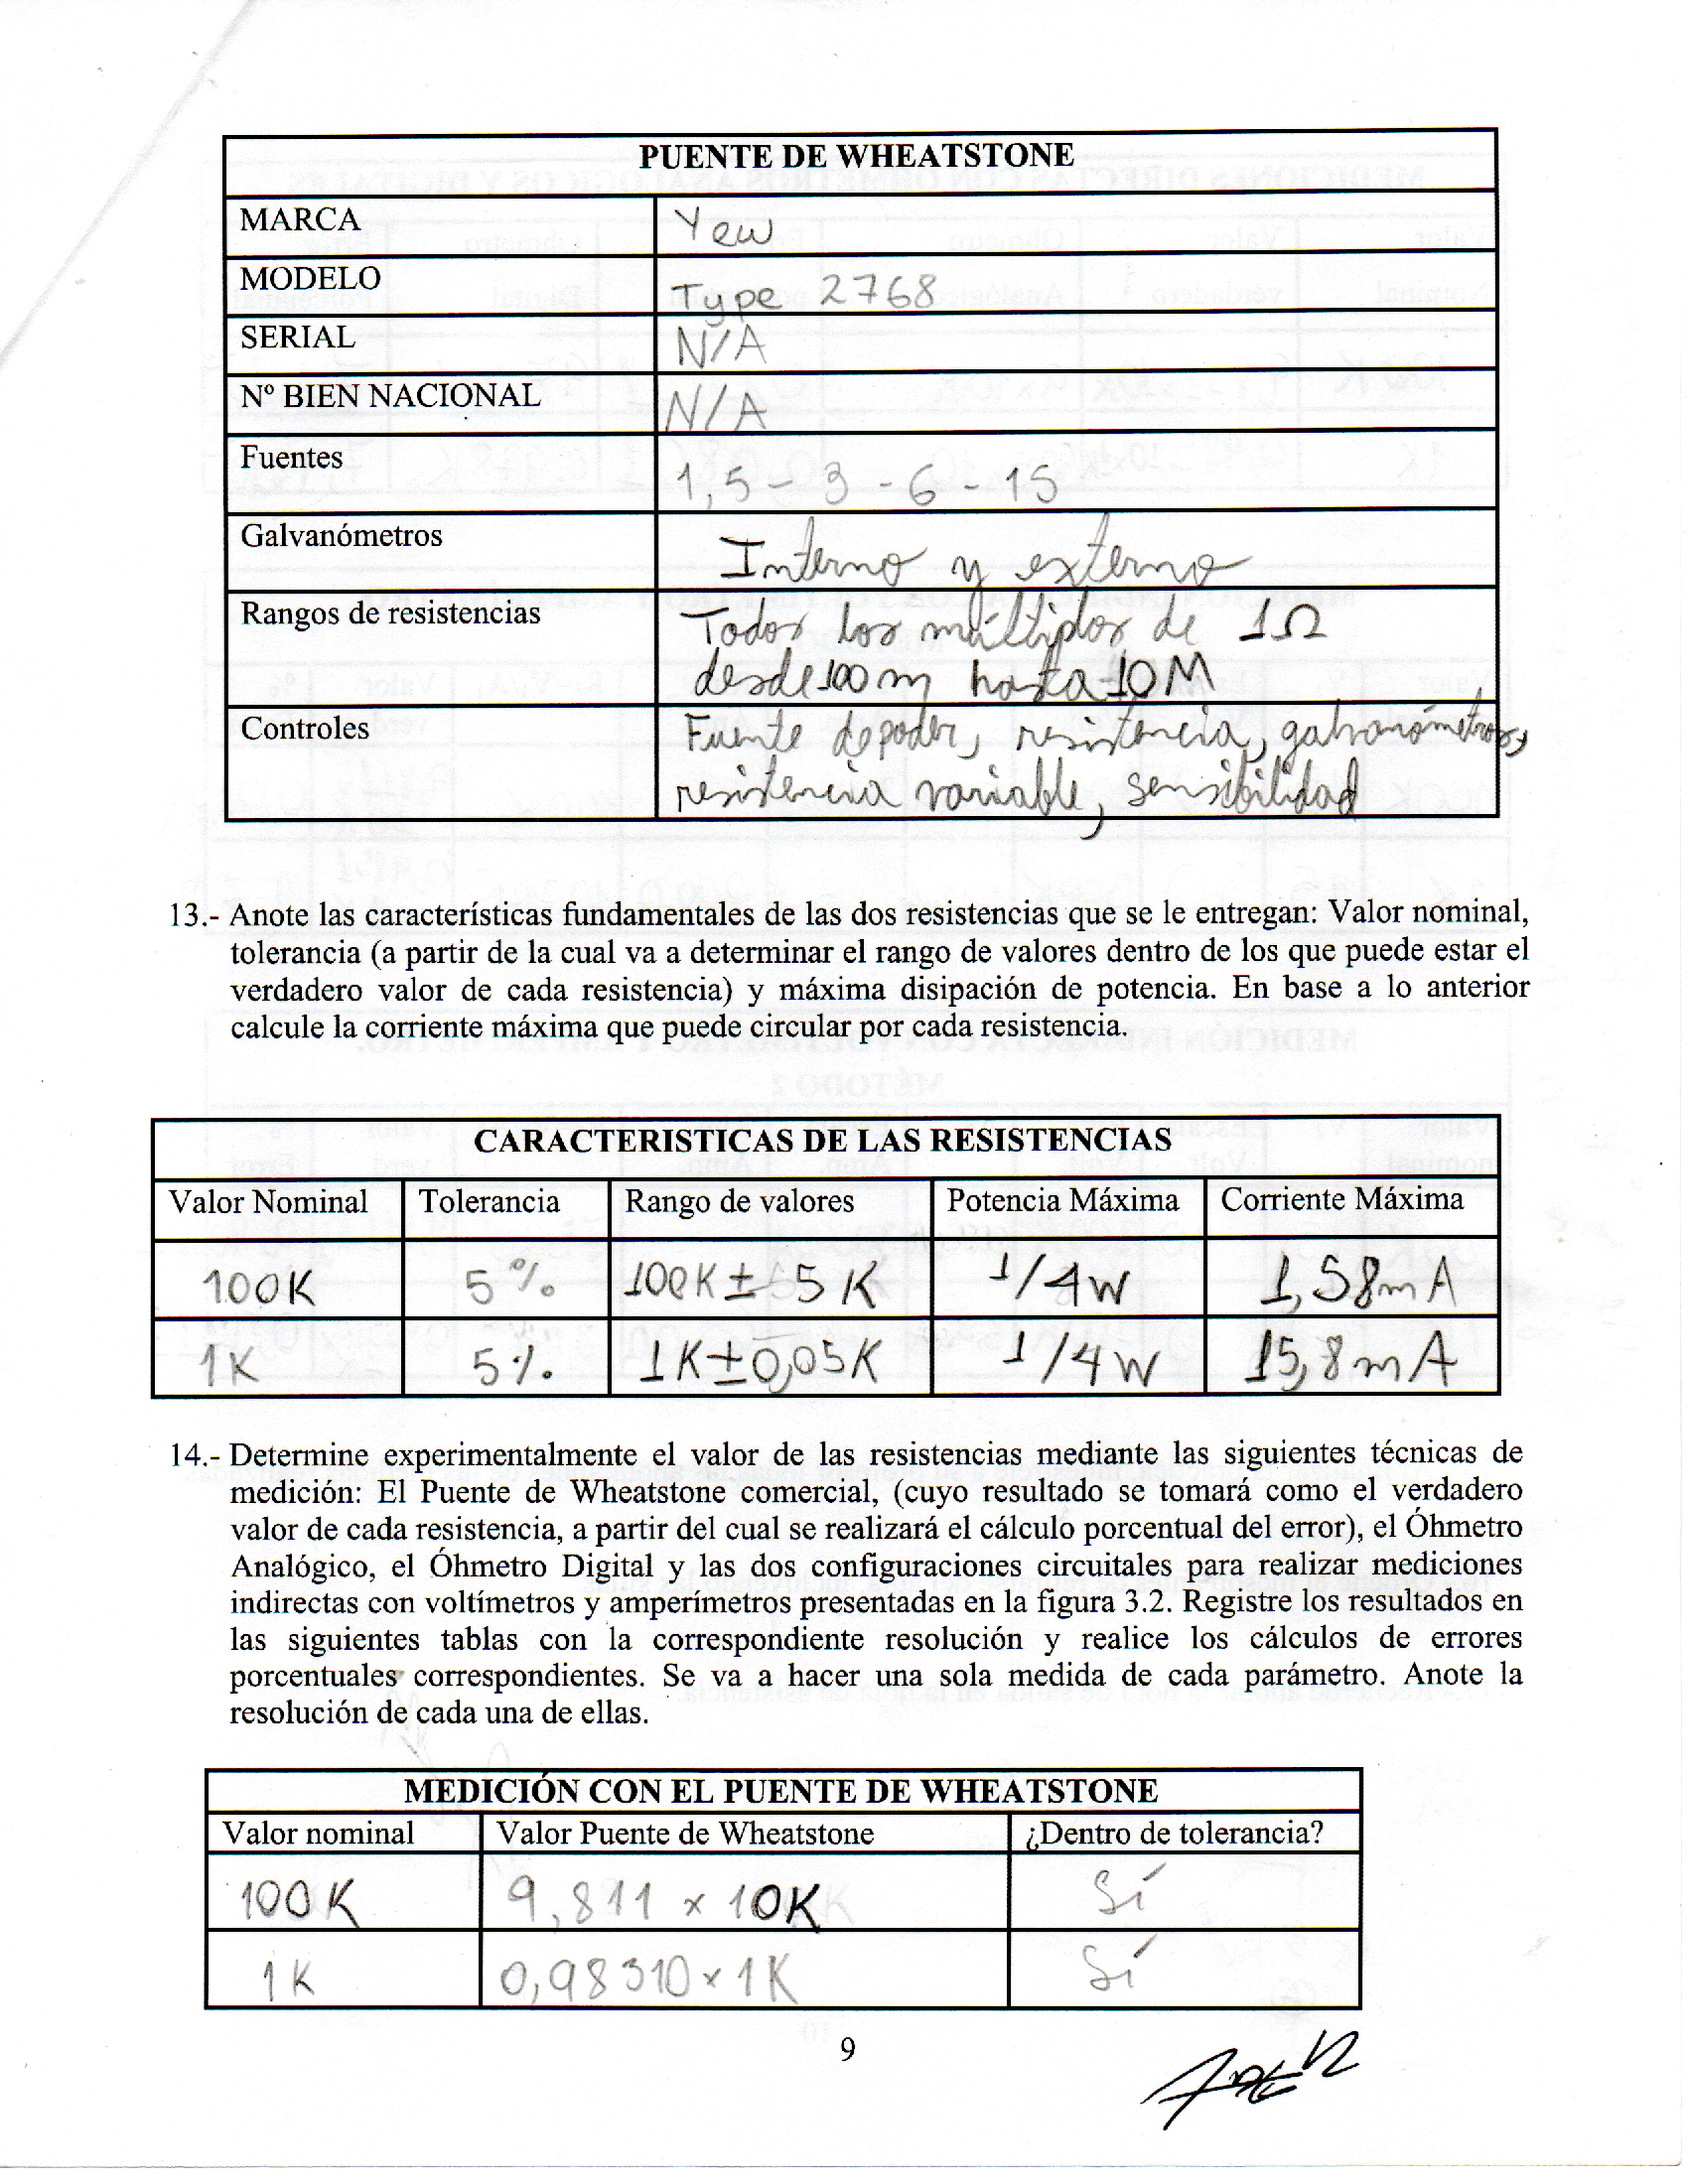
\includegraphics[width=16cm,height=20cm]{Img/datos_lab_0006}
	\end{center}

	\begin{center}
		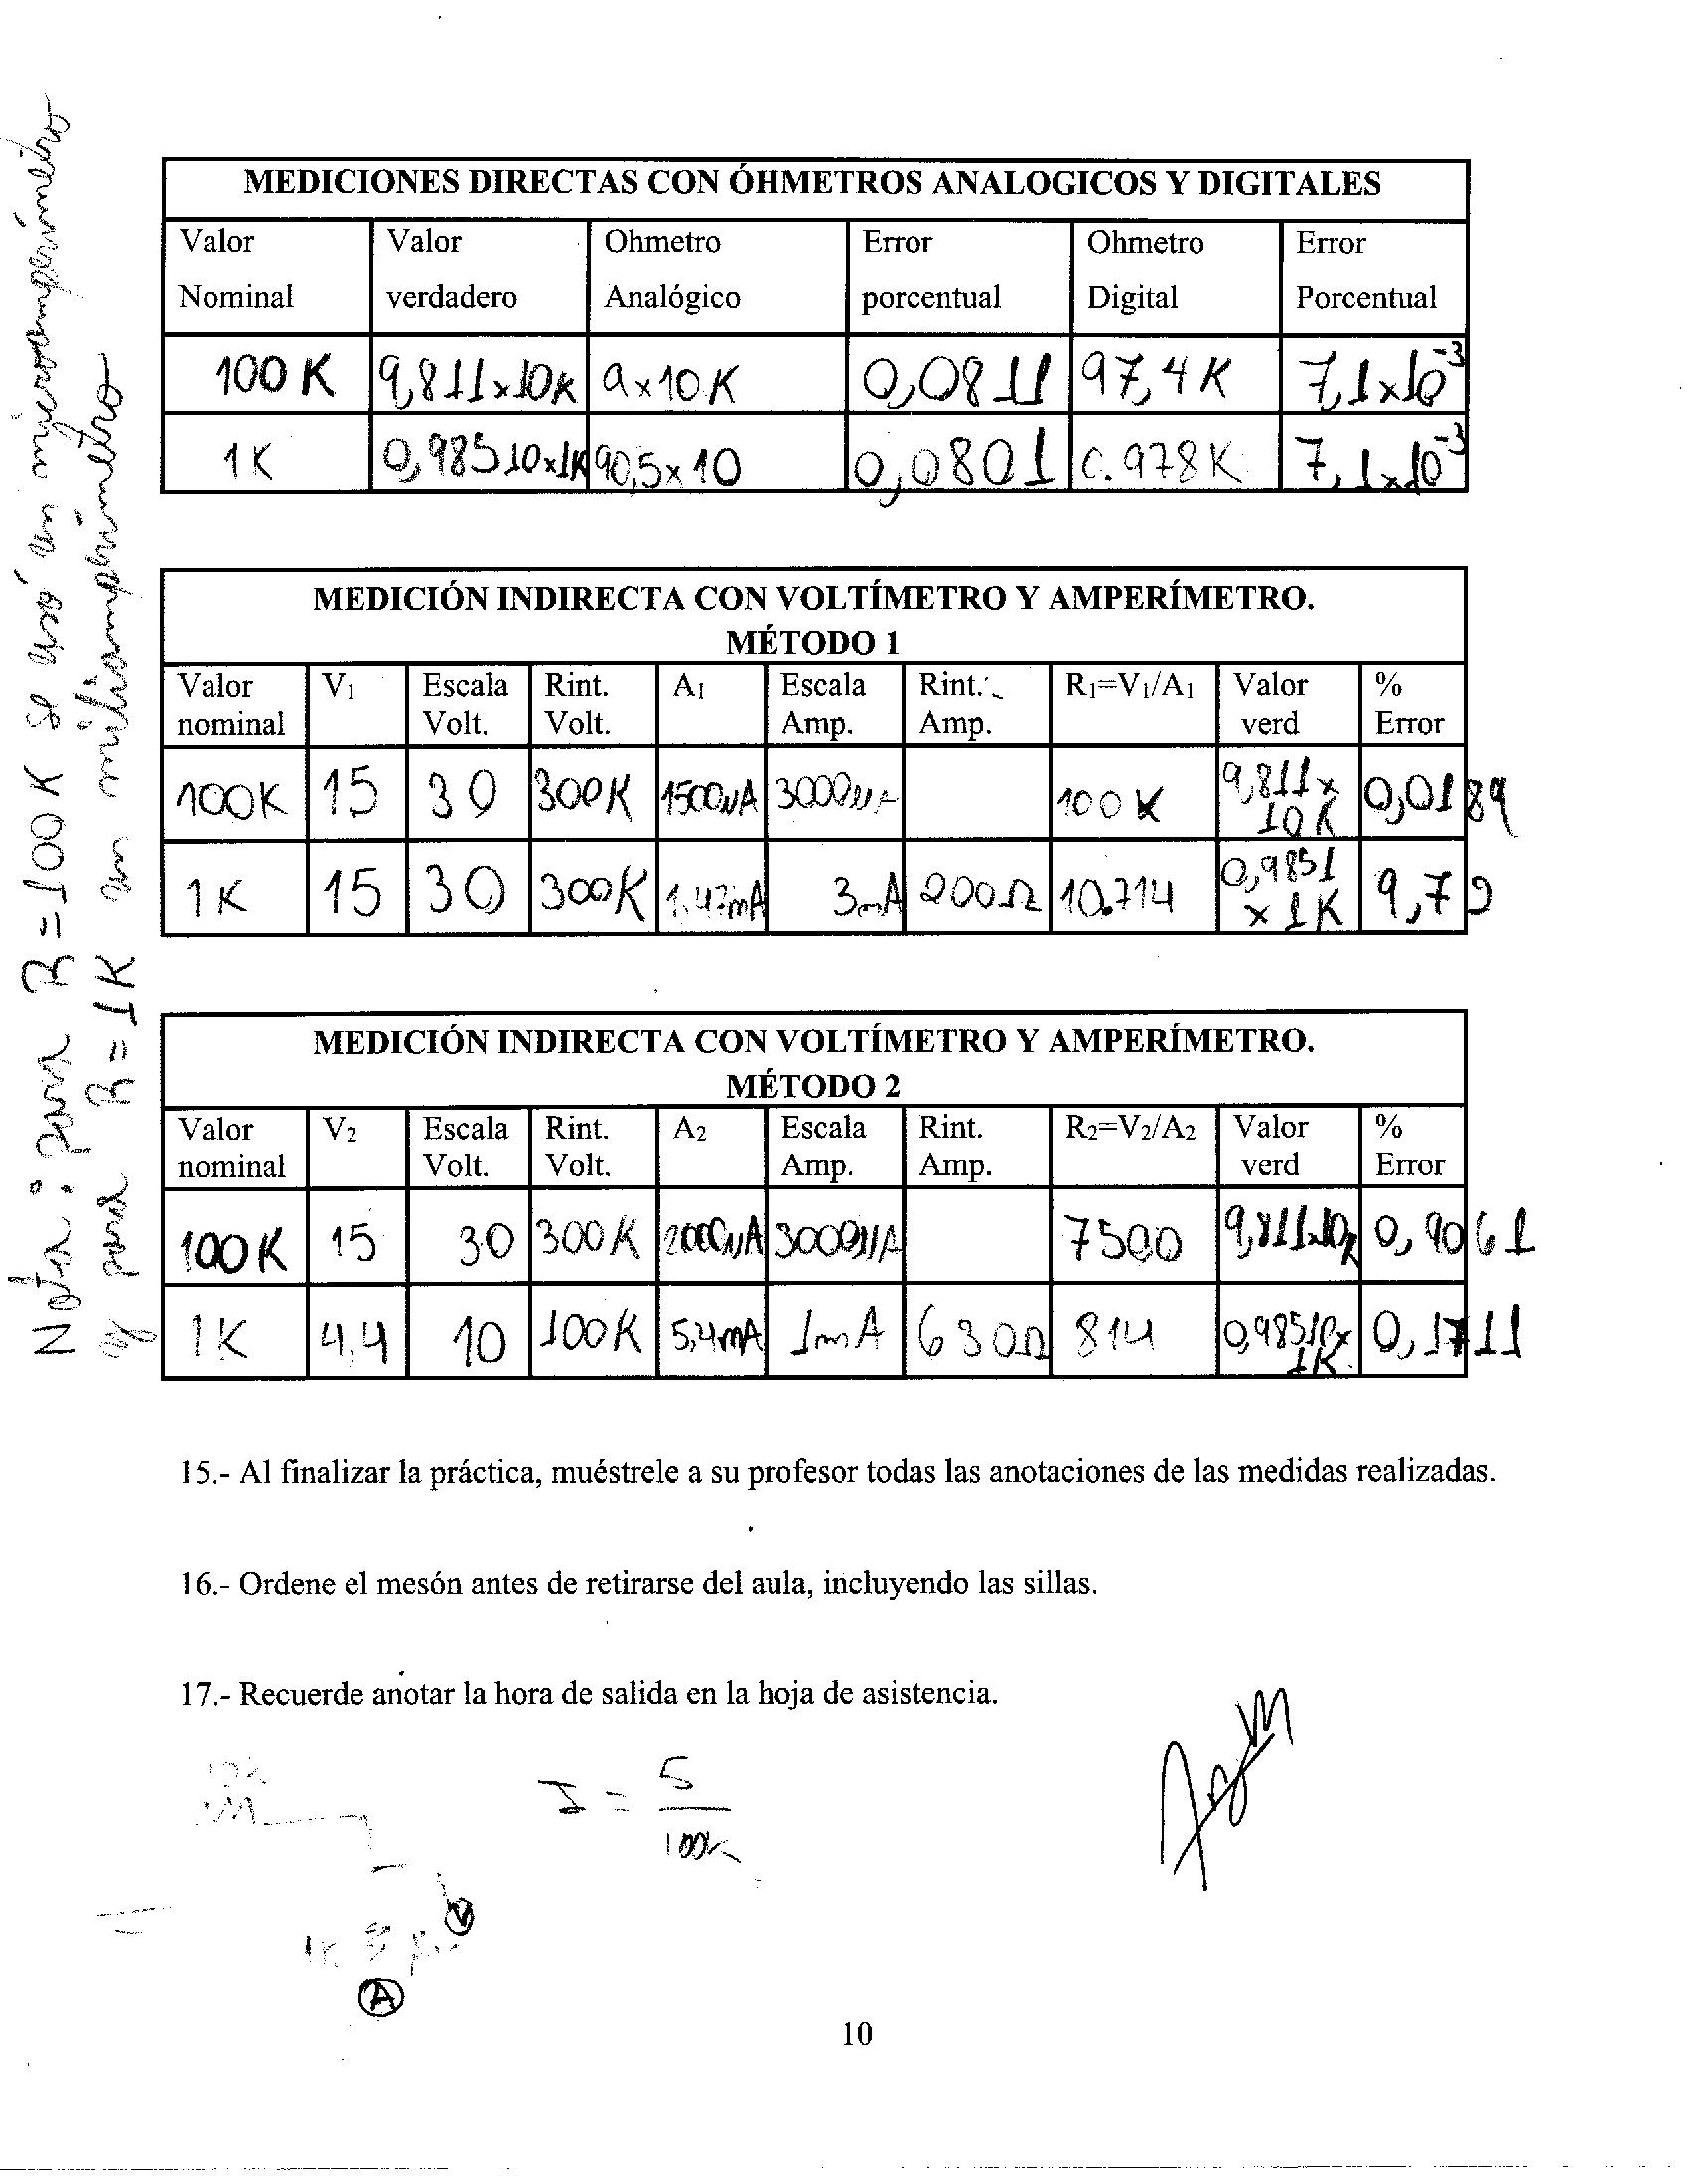
\includegraphics[width=16cm,height=20cm]{Img/datos_lab_0007}
	\end{center}

	\begin{center}
		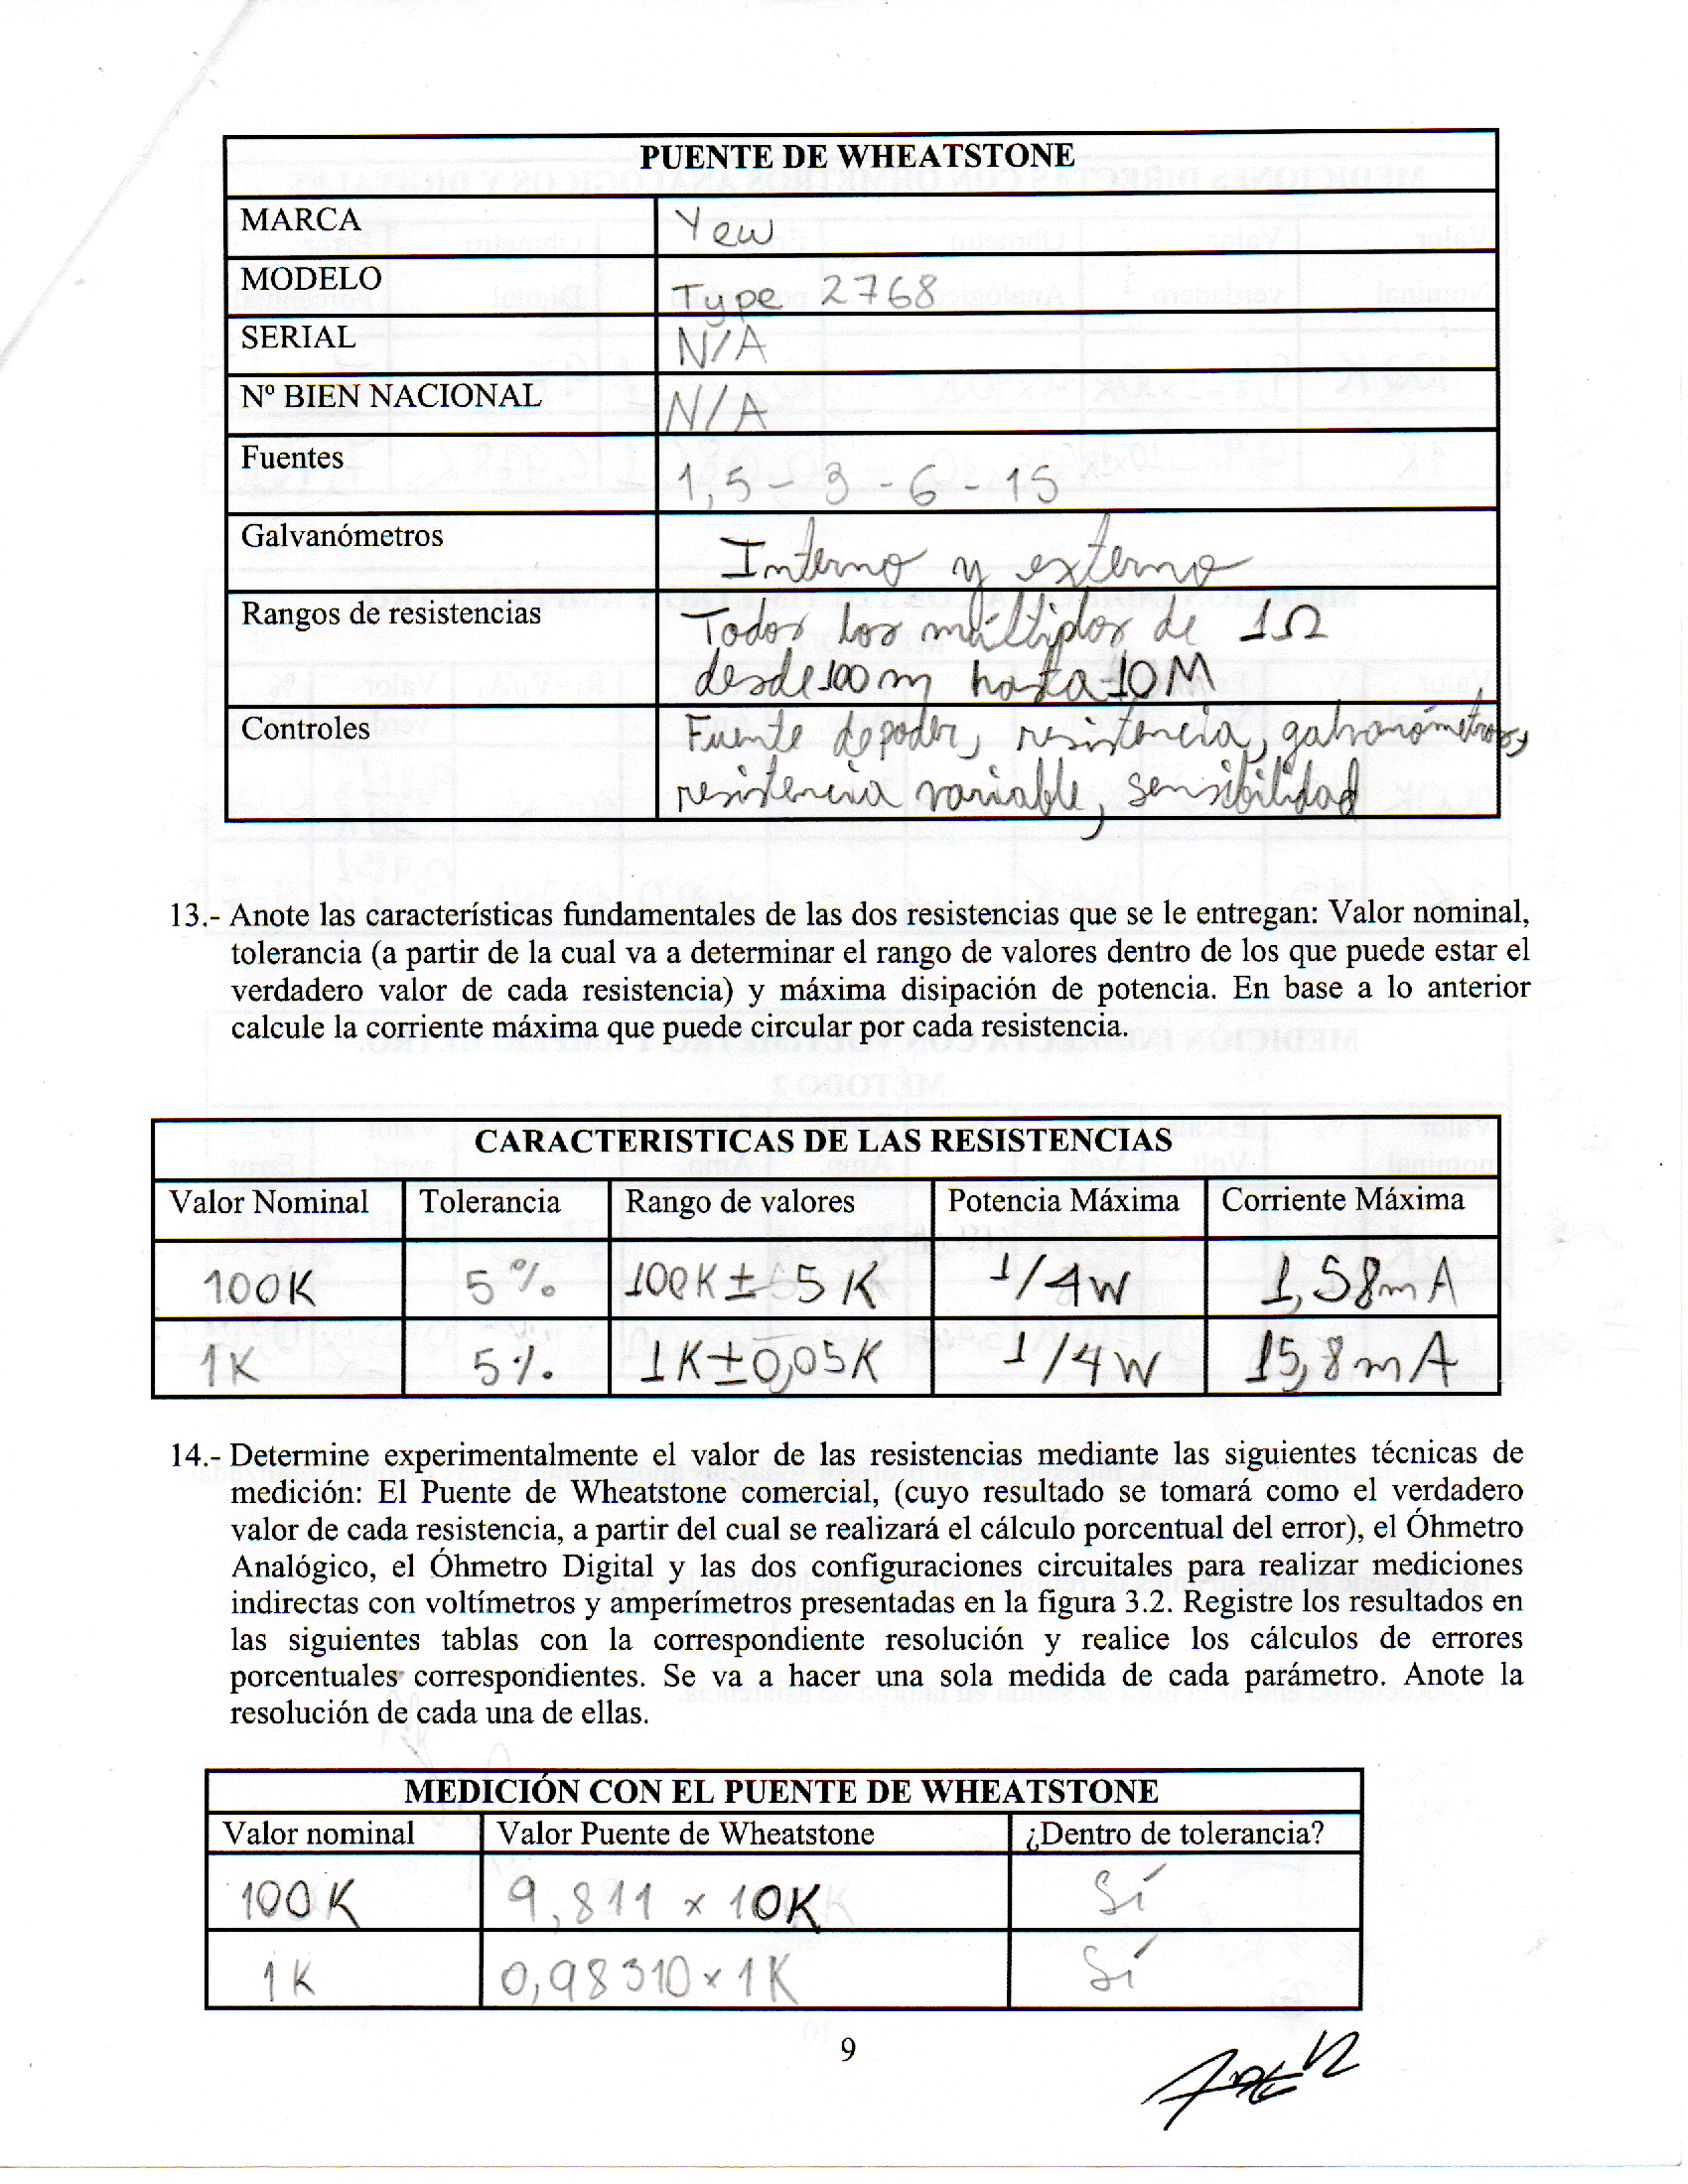
\includegraphics[width=16cm,height=20cm]{Img/datos_lab_0008}
	\end{center}

	\begin{center}
		\includegraphics[width=16cm,height=20cm]{Img/datos_lab_0009}
	\end{center}


	\newpage
	
	\begin{center}
		\textbf{\large ANÁLISIS DE RESULTADOS}\\
	\end{center}
	
	\section{Mediciones del amperímetro analógico}
	
	\noindent Según los resultados obtenidos hay que calcular las medidas de corriente del amperímetro analógico, ya que sólo se tomó la posición de la aguja, es decir que para la escala de $0,3mA$ se tendrá $I_j = \frac{0,3 \times n}{30}$ donde $n$ es la división en la que quedó la aguja, quedando $I_1 = 0,01mA$; $I_2 = 0,02mA$; $I_3 = 0,03mA$; $I_4 = 0,04mA$ para la escala de $0,3mA$. Para la escala de $1mA$ se tiene $I_j = \frac{1 \times n}{30}$,quedando $I_1 = 0,03mA$; $I_2 = 0,06mA$; $I_3 = 0,1mA$; $I_4 = 0,13mA$.\\
	
	\begin{center}
		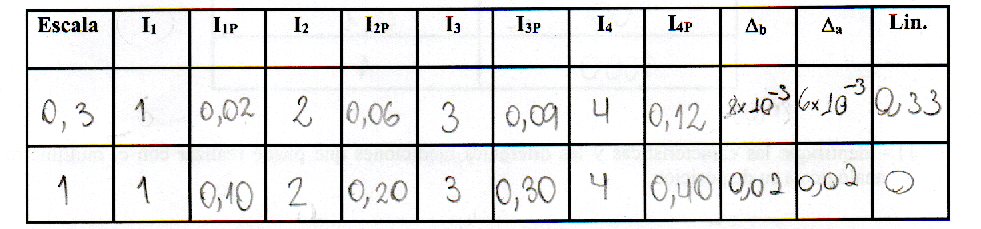
\includegraphics[width=16cm,height=3cm]{Img/anexo_1}
	\end{center}

	\noindent Se puede evidenciar a partir de los cálculos basados en los datos de la tabla anterior según los datos obtenidos es menos exacto que el amperímetro digital. Se cree que esto se debe a errores sistemáticos a la hora de realizar las mediciones por haberse equivocado en alguna parte del proceso de medición. Se estima que pobablemente el error radica en no haber subido lo suficiente al voltaje de la fuente para obtener medidas de las posiciones altas de la escala\\
	
	\noindent La precisión por otro lado, pese a cualquier error sistemático en el cual se haya podido incurrir, se nota que la precisión del amperímetro analógico es adecuada ya que refleja suficientes dígitos de la medida.\\
	
	\noindent Para la linealidad tendremos que en ambas escalas es cero, sin embargo, esto puede deberse al posible error mencionado anteriormente.
	
	\newpage
	
	\section{Mediciones de las resistencias mediante distintos métodos}
	
	\noindent Para este inciso se obtuvieron los siguientes datos:\\
	
	\begin{center}
		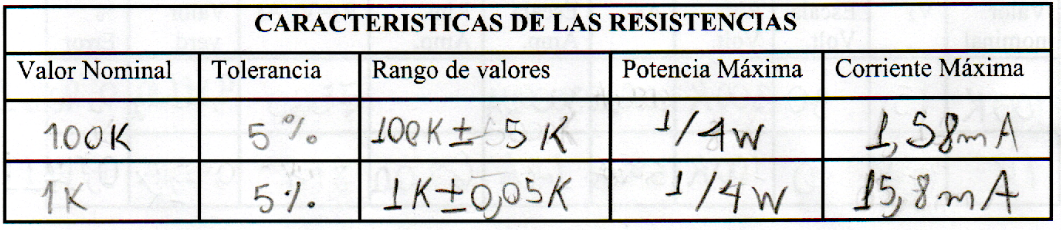
\includegraphics[width=16cm,height=3cm]{Img/anexo_2}
	\end{center}

	\begin{center}
		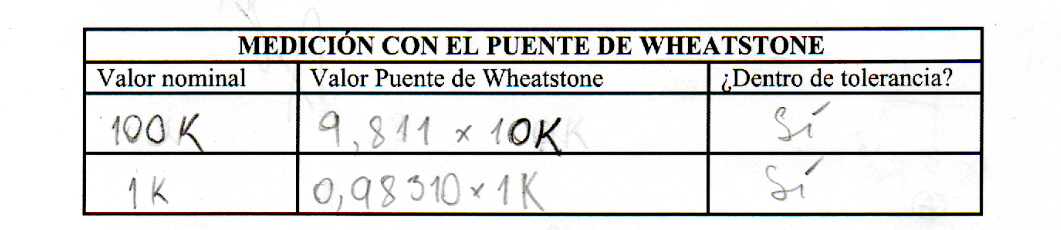
\includegraphics[width=16cm,height=3cm]{Img/anexo_3}
	\end{center}
	
	\begin{center}
		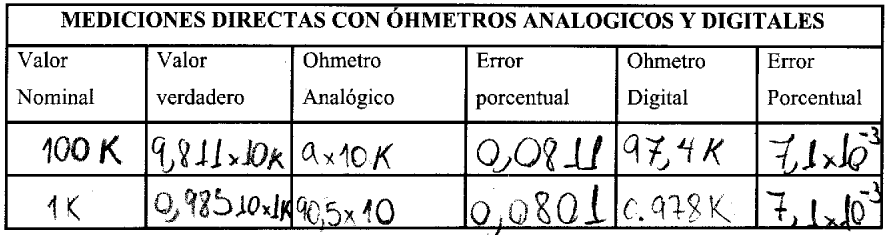
\includegraphics[width=16cm,height=3cm]{Img/anexo_4}
	\end{center}

	\begin{center}
		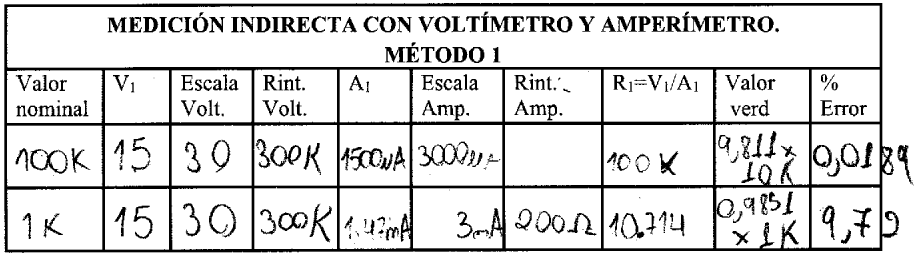
\includegraphics[width=16cm,height=3cm]{Img/anexo_5}
	\end{center}

	\begin{center}
		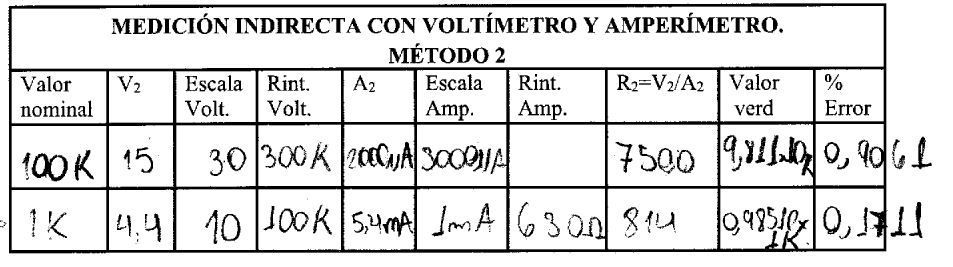
\includegraphics[width=16cm,height=3cm]{Img/anexo_6}
	\end{center}

	\noindent Se puede evidenciar que la medida más precisa y exacta fue la del puente de wheatstone ya que es un dispositivo diseñado específicamente para realizar medidas sumamente adecuadas.\\
	
	\noindent Para las mediciones directas se aprecia que el óhmetro digital es superior en cuanto a precisión y exactitud, destacando que el óhmetro analógico se sale del rango de valores de las resistencias en ambas medidas.\\
	
	\noindent En el primer método que consiste en el amperímetro en serie con la resistencia, se tiene que la resistencia de valor alto dió $100k\Omega$ lo cual es bastante preciso y está dentro del rango de valores de la resistencia, este resultado es sumamente cercano al medido con el puente de wheatstone. La resistencia de valor pequeño por otro lado resultó en un valor por encima de los $10k\Omega$ lo cual es totalmente erróneo y fuera del rango de valor.
	
	\noindent El segundo método consistió en el voltímetro en paralelo con la resistencia, quedando que para la resistencia alta su valor era $7,5k\Omega$, lo cual es errado totalmente, mientras que para la resistencia pequeña se tuvo que su valor fue de $814\Omega$ los cual es sumamente cercano, sin embargo, no se encuentra dentro del rango de valores de la resistencia.
	
	\noindent Estos resultados tienen sentido ya que se había determinado que para el primer método $R_x = \frac{V_{R_x}}{I_{R_x}} + R_{ia}$ y para el segundo $\frac{1}{R_x} = \frac{I_{R_x}}{V_{R_x}} + \frac{1}{R_{iv}}$. Esto sucede porque para el primer método, mientras más resistencia, menos afectará la resistencia interna del amperímetro que tiene en serie, mientras que en el segundo método la resistencia más pequeña no se verá gravemente afectada. Todo eso sucede porque la configuración en serie de resistencias las suma linealmente, mientras que en paralelo se suman sus inversos, es decir, la más pequeña definirá con mayor peso el resultado equivalente.\\
	
	\newpage
	
	\begin{center}
		\textbf{\large CONCLUSIONES}\\
	\end{center}
	
	Inserte conclusiones
	
	\newpage
	
\end{document}